% !TeX program = xelatex
% 按作者确认的全部完成状态修订。
% 英文统一使用 Times New Roman。
% 性能指标中的三张表使用 longtable，防止漂移到后续章节。

\documentclass[UTF8,a4paper,12pt,fontset=windows]{ctexart}

\usepackage[margin=2.5cm,top=3.2cm]{geometry}

\setmainfont{Times New Roman}
\setsansfont{Times New Roman}
\setmonofont{Times New Roman}

\usepackage{graphicx,eso-pic}
\usepackage{pdflscape}
\usepackage{float,caption,amsmath,needspace}
\usepackage{longtable,array,booktabs}
\usepackage[section]{placeins}
\usepackage{xurl}
\usepackage[hidelinks]{hyperref}

\urlstyle{same}

% 图、表编号
\renewcommand{\thefigure}{1-\arabic{figure}}
\renewcommand{\thetable}{1-\arabic{table}}

\captionsetup[figure]{
    font=small,
    labelsep=quad,
    skip=6pt
}

\captionsetup[table]{
    font=small,
    labelsep=quad,
    skip=6pt
}

% 页眉标志及下方横线：参照 Word 模板，每页均显示，包含首页。
\AddToShipoutPictureFG{%
    \AtPageUpperLeft{%
        \put(
            \LenToUnit{0.5\paperwidth},
            \LenToUnit{-15.0107mm}
        ){%
            \makebox[0pt][c]{%
                \raisebox{-\height}{%
                    \includegraphics[
                        width=65.1581mm,
                        height=11.9239mm
                    ]{images/header-logo.png}%
                }%
            }%
        }%
    }%
    \AtPageUpperLeft{%
        \put(
            \LenToUnit{0.5\paperwidth},
            \LenToUnit{-28.8mm}
        ){%
            \makebox[0pt][c]{\rule{\textwidth}{0.75pt}}%
        }%
    }%
}

\ctexset{
    section={
        beforeskip=0.9\baselineskip,
        afterskip=0.4\baselineskip
    },
    subsection={
        beforeskip=0.7\baselineskip,
        afterskip=0.3\baselineskip
    },
    subsubsection={
        beforeskip=0.6\baselineskip,
        afterskip=0.25\baselineskip
    }
}

\setlength{\intextsep}{8pt plus 2pt minus 2pt}
\setlength{\textfloatsep}{10pt plus 2pt minus 2pt}
\setlength{\parindent}{2em}
\setlength{\parskip}{0.25em}
\setlength{\emergencystretch}{4em}

\setlength{\LTpre}{0.3em}
\setlength{\LTpost}{0.5em}

\renewcommand{\arraystretch}{1.25}

% 避免为了撑满页面而过度拉大段落间距。
\raggedbottom

\begin{document}
\pagestyle{plain}

\begin{center}
    \Large\bfseries
    基于 FPGA-DPU 异构协同的红外视频增强与目标检测跟踪系统
\end{center}

\Needspace{3\baselineskip}
\section*{摘要}

针对红外图像存在对比度低、背景噪声干扰明显，以及实时视频处理对系统延迟和处理效率要求较高等问题，本文设计了一种基于 FPGA-DPU 异构协同的红外视频处理、目标检测与连续跟踪系统。系统以ZCU104 为硬件平台，以 FPGA PL端的视频流处理和图像预处理为核心，通过硬件流水线与并行处理提高图像处理效率，改善红外图像的视觉质量，为后续目标检测提供更适合的图 像输入，并结合间隔式目标检测与逐帧短时跟踪，实现红外目标的连续定位。

在 PL 端，系统以实时视频流处理为核心，构建涵盖视频输入、行场同步、图像统计、图像预处理、数据缓存及视频输出的完整硬件处理链路。针对红外图像动态范围有限、局部对比度不足及背景噪声干扰等问题，设计基于灰度统计的动态范围拉伸与局部细节增强方法，通过直方图统计、查找表、定点运算和行缓存等硬件结构，实现图像的高效流式处理。在此基础上，结合目标检测模型的输入要求，实现图像数据格式转换。同时，利用流水线并行处理和缓存管理机制，减少像素处理过程中的等待开销，保证视频流的连续传输与实时输出。针对两次目标检测之间的连续定位需求，在 PL 端实现基于绝对差和的单目标短时跟踪器，通过模板匹配与局部搜索逐帧更新目标位置，并结合误差和可信度判断目标状态，为后续检测触发和位置校正提供依据。

系统采用硬件适配、INT8量化并编译的YOLOv8n模型，DPU按预设帧间隔执行检测，输出目标类别、位置和置信度。跟踪可信度下降或目标丢失时，提前调用DPU重检，并据此校正位置、更新模板。间歇检测与逐帧跟踪相结合，减少对逐帧神经网络推理的依赖，提高处理速度。

针对视频输入与DPU推理速度不匹配造成的过期帧积压，设计基于三缓冲的Fresh-Frame调度，使DPU优先获取最新完整帧，并关联检测结果、跟踪状态和显示画面，避免延迟结果覆盖当前目标位置。该系统为资源受限环境下的红外视频智能处理提供可验证、可复现的实现方案。

关键词： 异构协同；红外视频处理；图像预处理；硬件流水线；目标检测

\clearpage
\section*{第一部分 作品概述}

\Needspace{3\baselineskip}
\section*{1.1 功能与特性}

本系统以 FPGA PL 端实时视频处理与图像预处理为核心，结合 DPU 间歇式目标检测，实现红外视频的实时处理、目标检测与连续跟踪。

\begin{enumerate}
    \item \textbf{实时视频处理：}
    实现视频流输入、行场同步、数据缓存及视频输出，采用硬件流水线与并行处理，提高视频处理效率，保障视频连续性。

    \item \textbf{图像预处理：}
    通过灰度统计、动态范围拉伸和局部细节增强，改善红外图像对比度；结合查找表、定点运算和行缓存，实现高效流式处理，并完成图像缩放、等比例填充及数据格式转换。

    \item \textbf{目标检测与连续跟踪：}
    利用 DPU 间隔式运行 YOLOv8n 完成目标检测，PL 通过 SAD 模板匹配逐帧更新目标位置，并在跟踪异常时触发重新检测，实现检测与跟踪协同。

    \item \textbf{低延迟帧调度：}
    采用 Frame ID 与三缓冲 Fresh-Frame 机制，优先处理最新完整帧，减少过期帧积压，并实现检测结果与视频画面的正确关联。
\end{enumerate}


\Needspace{3\baselineskip}
\section*{1.2 应用领域}

\begin{enumerate}
    \item \textbf{智能无人系统与边缘感知：}
    面向无人车、巡检机器人和无人值守终端，提供红外图像增强、目标检测与连续跟踪，支持夜间、弱光条件下的本地实时感知。

    \item \textbf{工业巡检与能源设施监测：}
    应用于变电站、能源场站及工业园区，对人员、车辆等目标进行持续定位与状态监测，辅助开展安全巡检和异常目标发现。

    \item \textbf{公共安全与应急救援：}
    用于夜间周界监测、道路目标观察和应急搜索，通过红外成像与连续跟踪，为值守人员提供目标位置及运动信息。

    \item \textbf{嵌入式视觉研究与教学：}
    作为FPGA硬件加速、深度学习部署和软硬件协同开发平台，通过更换模型与调整参数，扩展至其他红外目标感知任务。
\end{enumerate}


\Needspace{3\baselineskip}
\section*{1.3 主要技术特点}

\begin{enumerate}
    \item \textbf{FPGA与DPU异构协同：}
    摄像头直接接入PL，利用硬件流水线与并行运算完成视频处理；DPU执行神经网络推理，PS负责配置、调度及后处理，实现任务分工。

    \item \textbf{流式预处理与双反馈增强：}
    结合非均匀性校正、场景统计和空间自适应增强改善红外图像质量，以跟踪可信度和检测结果形成双反馈，增强参数在帧首统一更新。

    \item \textbf{间歇检测与逐帧跟踪：}
    采用YOLOv8n INT8模型按需检测，结合PL端SAD模板匹配连续更新目标位置，在跟踪异常时触发重检，降低逐帧推理开销。

    \item \textbf{新鲜帧调度与结果对齐：}
    采用三缓冲优先处理最新完整帧，通过帧号、缓冲编号、复用代次及原子提交保护数据一致性；显示缓存独立管理，避免旧结果误用。
\end{enumerate}


\Needspace{3\baselineskip}
\section*{1.4 主要性能指标}

% 以下数值为示例数据，并非项目实测结果。
% 三张表全部采用非浮动的longtable，允许跨页并重复表头。

\Needspace{5\baselineskip}
\subsection*{不同优化方法的帧率与延迟对比}

\begingroup
\small
\setlength{\tabcolsep}{5pt}
\renewcommand{\arraystretch}{1.3}

\begin{longtable}{
    >{\raggedright\arraybackslash}p{0.43\linewidth}
    ccc
}
\caption{不同优化方法的帧率与显示延迟对比（示例数据，非实测）}
\label{tab:fps_latency}\\

\toprule
处理方法 & 检测帧率 & 连续定位帧率 & 显示延迟 \\
\midrule
\endfirsthead

\multicolumn{4}{c}{\small 表\thetable（续）}\\[4pt]
\toprule
处理方法 & 检测帧率 & 连续定位帧率 & 显示延迟 \\
\midrule
\endhead

\midrule
\multicolumn{4}{r}{\footnotesize 接下页}\\
\endfoot

\bottomrule
\endlastfoot

纯DPU检测
& 12 FPS & 12 FPS & 180 ms \\

DPU检测 + 三缓冲
& 15 FPS & 15 FPS & 100 ms \\

DPU检测 + SAD跟踪
& 12 FPS & 30 FPS & 80 ms \\

DPU检测 + SAD跟踪 + 三缓冲
& 15 FPS & 30 FPS & 55 ms \\

空间增强 + DPU检测
& 11 FPS & 11 FPS & 190 ms \\

空间增强 + DPU检测 + SAD跟踪
& 11 FPS & 30 FPS & 90 ms \\

空间增强 + DPU检测 + SAD跟踪 + 三缓冲
& 14 FPS & 30 FPS & 65 ms \\

\end{longtable}
\endgroup

\noindent
表中显示延迟指摄像头采集至对应标注画面显示的平均延迟。
检测帧率统计包含张量准备、推理和后处理的完整检测服务；
连续定位帧率统计有效目标位置的更新频率。
三缓冲用于改善处理重叠和新鲜帧供给，具体收益以实测为准。


\Needspace{5\baselineskip}
\subsection*{不同优化方法的精度及提升幅度对比}

\begingroup
\footnotesize
\setlength{\tabcolsep}{3pt}
\renewcommand{\arraystretch}{1.35}

\begin{longtable}{
    >{\raggedright\arraybackslash}p{0.32\linewidth}
    cccccc
}
\caption{检测精度与定位成功率对比（示例数据，非实测）}
\label{tab:accuracy_improvement}\\

\toprule
处理方法
& Precision
& Recall
& mAP@0.5
& 定位成功率
& mAP提升
& 定位提升 \\
\midrule
\endfirsthead

\multicolumn{7}{c}{\small 表\thetable（续）}\\[4pt]
\toprule
处理方法
& Precision
& Recall
& mAP@0.5
& 定位成功率
& mAP提升
& 定位提升 \\
\midrule
\endhead

\midrule
\multicolumn{7}{r}{\footnotesize 接下页}\\
\endfoot

\bottomrule
\endlastfoot

纯DPU检测
& 85\% & 82\% & 80\% & 88\% & 基准 & 基准 \\

DPU检测 + 三缓冲
& 85\% & 82\% & 80\% & 88\% & 0 & 0 \\

DPU检测 + SAD跟踪
& 85\% & 82\% & 80\% & 95\% & +0 & +7 \\

DPU检测 + SAD跟踪 + 三缓冲
& 85\% & 82\% & 80\% & 95\% & +0 & +7 \\

空间增强 + DPU检测
& 92\% & 89\% & 88\% & 91\% & +8 & +3 \\

空间增强 + DPU检测 + SAD跟踪
& 92\% & 89\% & 88\% & 96\% & +8 & +8 \\

空间增强 + DPU检测 + SAD跟踪 + 三缓冲
& 92\% & 89\% & 88\% & 96\% & +8 & +8 \\

\end{longtable}
\endgroup

\noindent
提升幅度均相对于纯DPU检测，单位为百分点。
检测精度在固定图像测试集上评价，连续定位成功率按视频逐帧评价，
成功帧定义为预测框与标注框的IoU不低于0.5。
三缓冲不直接改变模型输出，因此示例中不为其设置额外检测精度收益；
其主要作用通过帧率、延迟和结果帧龄体现。


\Needspace{5\baselineskip}
\subsection*{视频输入输出与主要事件响应时间}

\begingroup
\small
\setlength{\tabcolsep}{4pt}
\renewcommand{\arraystretch}{1.3}

\begin{longtable}{
    >{\raggedright\arraybackslash}p{0.27\linewidth}
    >{\raggedright\arraybackslash}p{0.49\linewidth}
    c
}
\caption{主要处理阶段与事件响应时间（示例数据，非实测）}
\label{tab:response_time}\\

\toprule
处理阶段或事件 & 计时起止点 & 示例时间 \\
\midrule
\endfirsthead

\multicolumn{3}{c}{\small 表\thetable（续）}\\[4pt]
\toprule
处理阶段或事件 & 计时起止点 & 示例时间 \\
\midrule
\endhead

\midrule
\multicolumn{3}{r}{\footnotesize 接下页}\\
\endfoot

\bottomrule
\endlastfoot

摄像头输入帧周期
& 相邻两帧SOF之间，输入为30 FPS。
& 33.3 ms \\

PL预处理附加延迟
& 同一有效像素进入预处理链至对应像素输出。
& 2 ms \\

SAD逐帧位置更新
& 当前帧跟踪所需像素就绪至目标位置发布。
& 3 ms \\

三缓冲帧发布
& DDR成功写入状态被接收至对应槽发布为READY。
& 0.1 ms \\

检测请求调度
& DPU空闲且存在READY帧至PS开始处理请求。
& 1 ms \\

输入张量准备
& PS开始读取锁定帧至模型输入张量就绪。
& 6 ms \\

DPU推理
& 推理任务提交至模型输出张量可用。
& 55 ms \\

解码、NMS与坐标还原
& 模型输出可用至原图坐标检测结果形成。
& 5 ms \\

结果原子提交
& 后处理完成至PL接受完整结果及身份字段。
& 1 ms \\

显示帧发布等待
& 完整显示帧就绪至下一输出SOF发布。
& 0--16.7 ms \\

连续跟踪画面端到端延迟
& 摄像头采集至对应增强、跟踪和标注画面显示。
& 65 ms \\

首次有效目标识别
& 目标首次进入有效画面至首次有效检测结果发布。
& 80--120 ms \\

跟踪异常后的重检响应
& 重检请求被接受至新的检测结果提交。
& 70--100 ms \\

无目标结果处理
& 推理正常完成且无有效框至无目标状态发布。
& 1 ms \\

输入异常状态上报
& 接入模块确认边界或协议错误至错误状态可读。
& 1 ms \\

异常恢复至有效视频
& 启动受控恢复至重新接收并发布完整有效帧。
& 100--300 ms \\

\end{longtable}
\endgroup

\noindent
摄像头帧周期、流水线附加延迟和事件响应时间具有不同计时口径，
各行不能直接相加。无目标属于正常检测结果，不作为设备故障；
重检响应时间还受检测周期、资源占用及完整帧可用时间影响。


% 在进入1.5之前，确保前面的浮动对象已经排完。
\FloatBarrier
\Needspace{4\baselineskip}
\section*{1.5 主要创新点}

\begin{enumerate}
    \item \textbf{任务感知双反馈增强：}
    融合跟踪可信度与检测结果，动态调整红外增强参数，兼顾视觉质量与检测需求。

    \item \textbf{检测跟踪异构协同：}
    结合DPU间歇检测与PL逐帧SAD跟踪，降低连续定位对逐帧神经网络推理的依赖。

    \item \textbf{新鲜帧三缓冲调度：}
    优先处理最新完整帧，利用帧号、缓冲代次和原子提交减少积压与过期结果误用。

    \item \textbf{检测显示独立管理：}
    分离检测帧池与显示缓存，实现连续输出及目标标注的帧身份对齐。
\end{enumerate}


\Needspace{4\baselineskip}
\FloatBarrier
\section*{1.6 设计流程}



% PPT P1
\begin{figure}[H]
    \centering
    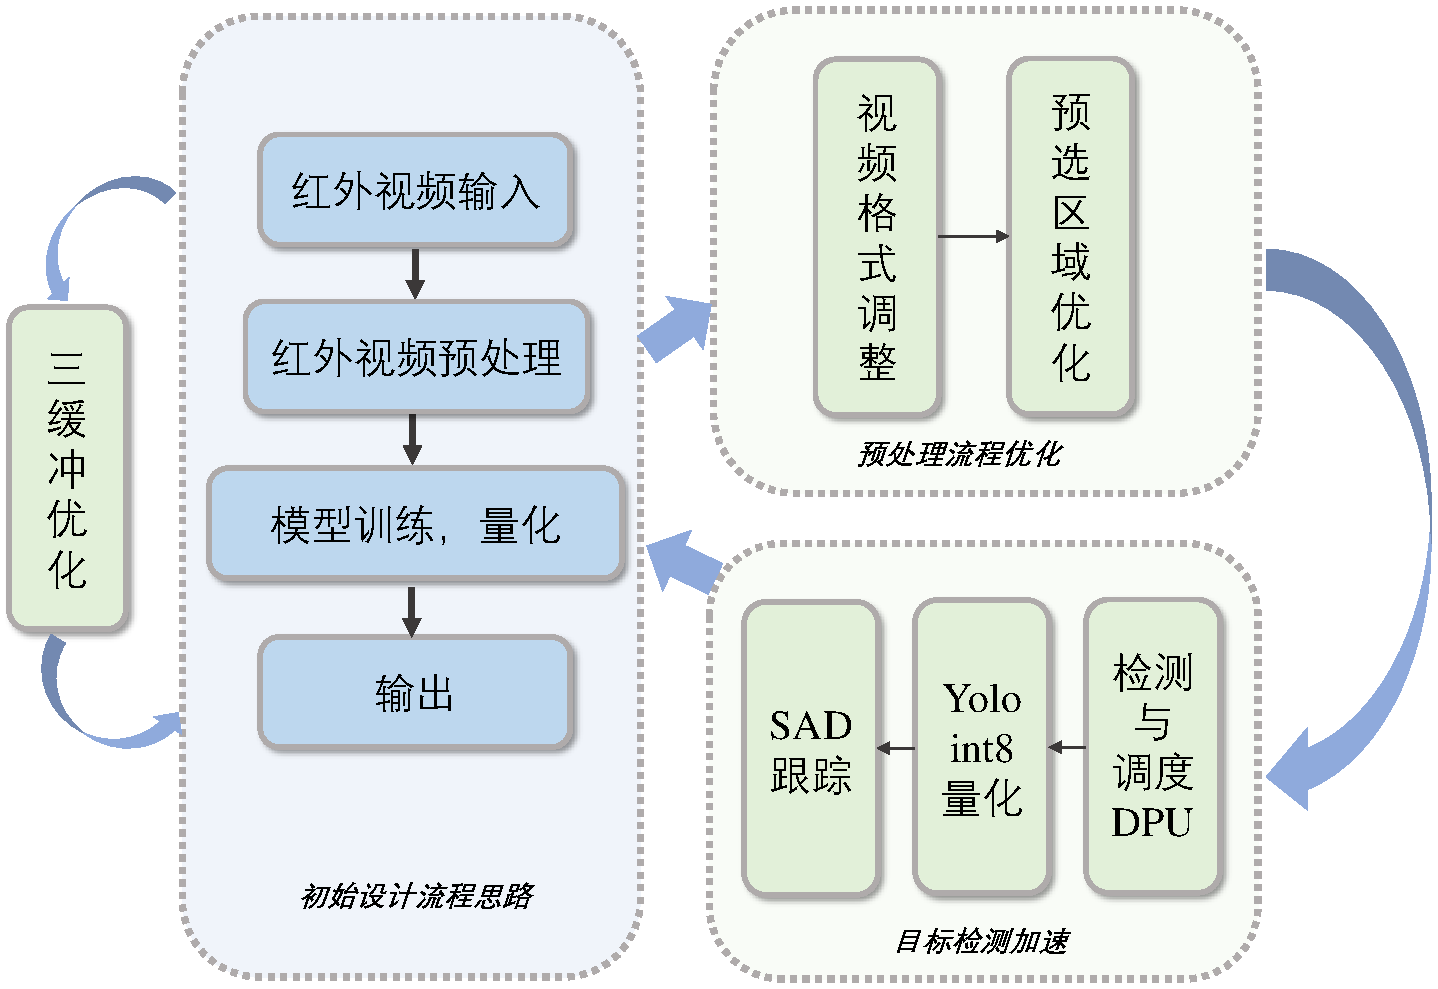
\includegraphics[
        width=0.66\linewidth,
        height=0.38\textheight,
        keepaspectratio
    ]{images/flowcharts/p01.pdf}
    \caption{设计流程图}
    \label{fig:design}
\end{figure}
\begin{enumerate}
    \item 完成摄像头红外视频接入与基础预处理，部署训练、量化后的YOLOv8n模型，通过DPU实现目标检测。

    \item 为提高检测精度，进一步加入空间自适应增强与候选区域优化，改善目标对比度。

    \item 为提高连续跟踪帧率，结合PL端SAD逐帧跟踪与DPU按需检测调度，利用检测结果初始化和校正跟踪。

    \item 最后引入新鲜帧三缓冲，减少旧帧积压，实现检测精度、跟踪帧率与处理延迟的协同优化。
\end{enumerate}


\Needspace{3\baselineskip}
\section*{第二部分 系统组成及功能说明}

\Needspace{3\baselineskip}
\section*{2.1 整体介绍}

系统以摄像头输入的连续红外视频为主线，通过PL预处理、检测与跟踪协同以及标注显示形成完整闭环。摄像头像素经采集、帧同步和时钟域转换后，统一为640×480 GRAY8视频流，依次进入图像校正、场景统计和空间自适应增强模块。增强后的图像在PL内分路：一路保持原尺寸，连续送入SAD跟踪与显示链路；另一路经Letterbox转换，由DataMover写入检测三缓冲，为DPU提供最新完整帧。由此，连续跟踪与间歇检测共享同一图像来源，并按各自节奏并行运行。

当达到检测周期或跟踪状态异常时，PL发布检测请求，PS根据请求中的帧身份读取锁定图像并调用DPU，完成解码、NMS和坐标还原后，将检测结果回写PL。目标状态机结合来源帧信息与当前跟踪状态，完成目标初始化、位置校正或重新检测，并将有效目标信息送往OSD，与对应视频画面关联后输出。同时，跟踪可信度形成快反馈，检测结果形成慢反馈，两路信息共同作用于双反馈控制器，调整后续增强参数与检测调度，参数在帧首统一锁存。

整个系统通过统一帧身份连接图像流、检测结果和跟踪状态，通过检测三缓冲与独立显示缓存协调不同处理速度，使图像预处理、目标定位、反馈控制和视频输出相互衔接，构成持续运行的红外视觉处理系统。

% PPT P2
\begin{figure}[H]
    \centering
    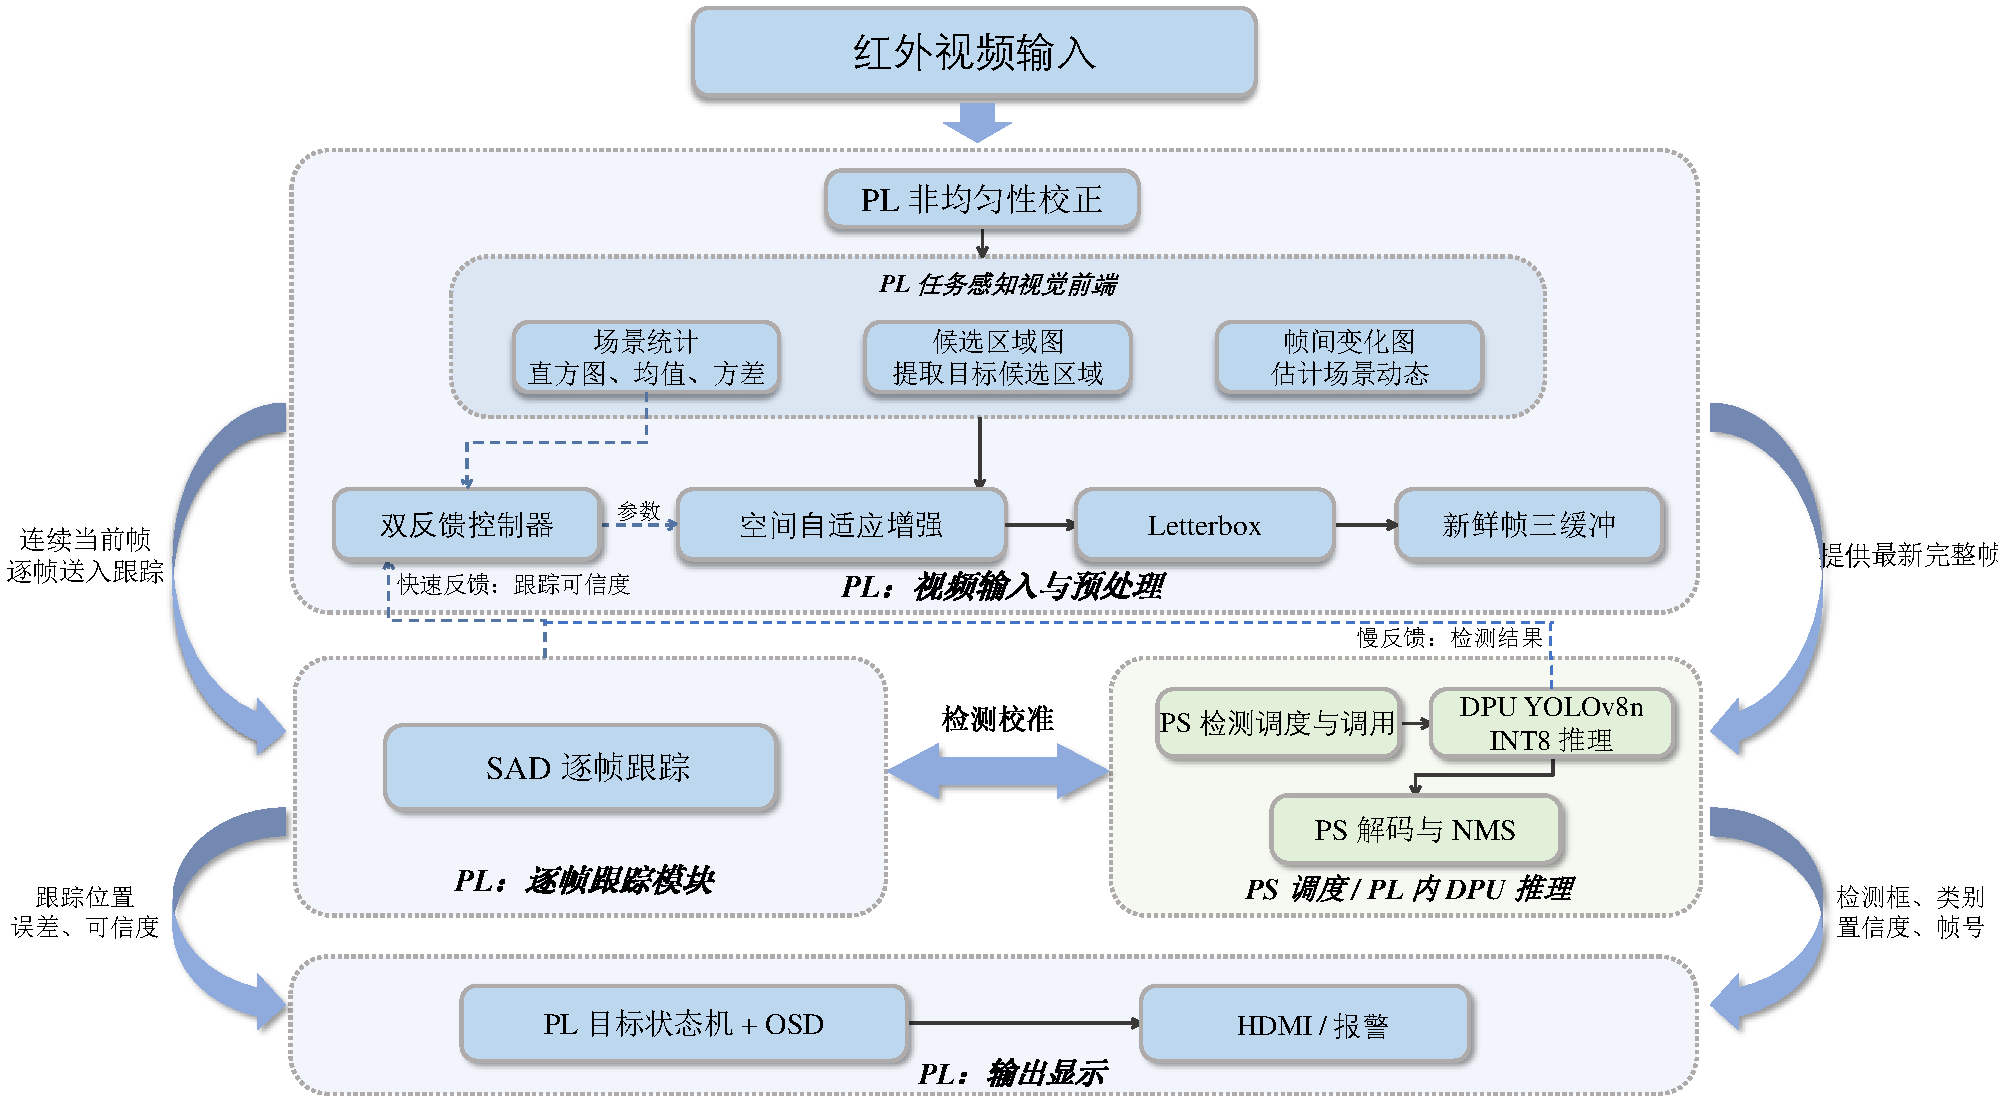
\includegraphics[
        width=\linewidth,
        height=0.60\textheight,
        keepaspectratio
    ]{images/flowcharts/p02.pdf}
    \caption{系统总体方案图}
    \label{fig:overall}
\end{figure}



\Needspace{3\baselineskip}
\section*{2.2 硬件系统介绍}

\Needspace{3\baselineskip}
\subsection*{2.2.1 硬件整体介绍}

硬件以ZCU104及其Zynq UltraScale+ MPSoC为核心，利用片上处理系统PS、可编程逻辑PL与共享DDR构建红外视频处理架构。如图~\ref{fig:hardware}~所示，红外摄像头直接向PL提供连续像素流，PS通过控制接口完成摄像头参数及硬件寄存器配置，使视频采集、图像处理和检测调度在统一控制下运行。图像数据主要沿PL处理链和DDR存储通路传输，PS承担配置与任务协调，形成数据处理与控制管理相互配合的硬件结构。
% PPT P3
\begin{figure}[H]
    \centering
    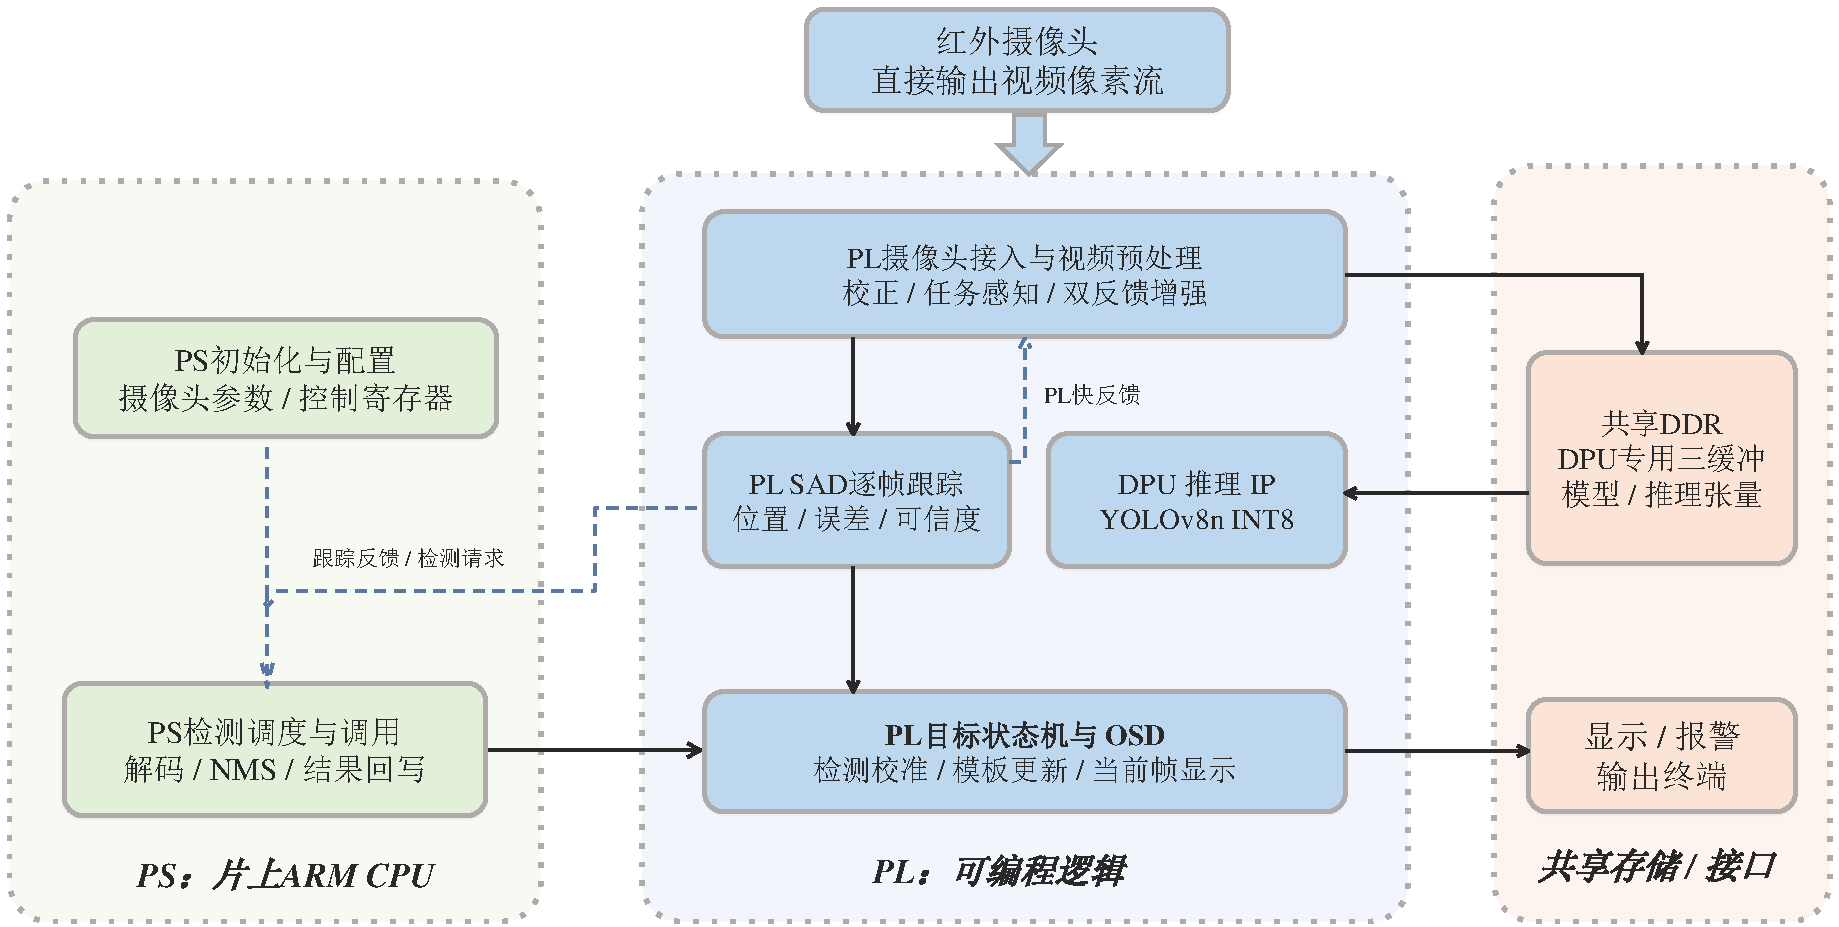
\includegraphics[
        width=\linewidth,
        height=0.60\textheight,
        keepaspectratio
    ]{images/flowcharts/p03.pdf}
    \caption{系统硬件总体架构图}
    \label{fig:hardware}
\end{figure}

摄像头视频进入PL后，依次完成接入同步、图像校正、任务感知和双反馈增强，随后分为连续跟踪与目标检测两条支路。原尺寸增强图像直接送入SAD模块，逐帧产生目标位置、匹配误差和跟踪可信度；检测支路经Letterbox转换后写入共享DDR中的DPU专用三缓冲。部署于PL侧的DPU读取完整检测帧及模型数据，执行YOLOv8n INT8推理。共享DDR连接预处理写入端与推理读取端，通过缓冲状态和所有权管理协调两者的处理速度，避免正在检测的图像被新帧覆盖。

SAD输出一方面进入目标状态机，维持连续目标定位，另一方面形成返回预处理链的快速反馈，并为PS检测调度提供依据。PS调用DPU并完成解码、NMS和结果回写后，检测结果进入PL目标状态机，与来源帧身份及跟踪状态关联，完成位置校正和模板更新。状态机再将有效目标信息交给OSD，与对应视频画面叠加后送至显示或报警终端。由此，摄像头、PL处理链、共享DDR、DPU与PS控制通路相互连接，形成连续采集、并行检测跟踪、反馈校正及标注输出的硬件闭环。


\Needspace{3\baselineskip}
\subsection*{2.2.2 机械设计介绍}

本作品已完成由标准开发板、红外摄像头和显示终端构成的原型安装。机械部分采用板卡与外围设备的固定和布线方案，满足摄像头视轴稳定、接口可靠、供电连接和板卡散热要求。系统采用标准ZCU104板卡，工程成果体现为原型安装与系统连接。

安装时保证摄像头视轴稳定、接口固定和线缆应力释放；开发板周围保留供电接线与散热空间，使风扇和散热片无遮挡。摄像头供电、电平与连接器按实际器件规格匹配，板卡和显示终端布线避免妨碍散热及调试。原型已完成设备固定、线缆整理与运行检查，接线位置和设备布局便于观察输入画面、显示结果及调试状态。


\Needspace{3\baselineskip}
\subsection*{2.2.3 电路各模块介绍}
\subsubsection*{（1）摄像头接入与 PL 视频预处理电路}

\begin{figure}[H]\centering
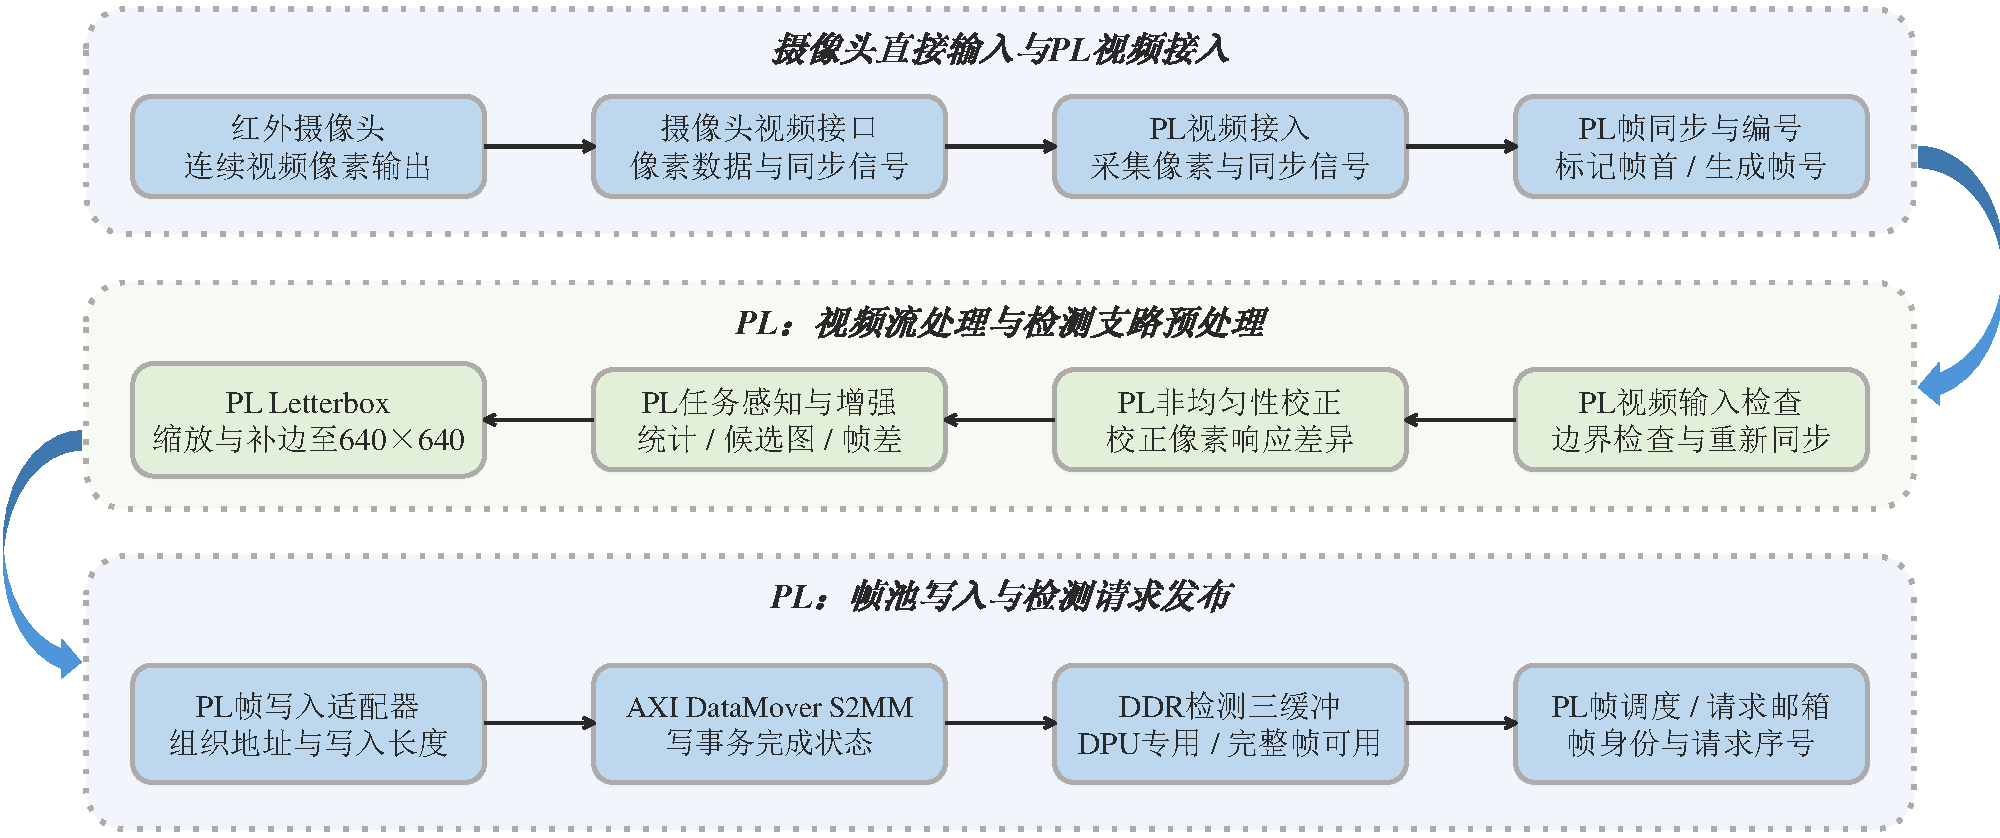
\includegraphics[width=\linewidth,height=0.58\textheight,keepaspectratio]{images/flowcharts/p05.pdf}
\caption*{图2-1 摄像头接入与 PL 预处理总体连接图}
\end{figure}

\paragraph*{1. 摄像头接入与 PL 预处理总体连接}
如图2-1所示，摄像头接入与 PL 视频预处理电路是系统前端的核心硬件部分，主要负责红外视频采集、视频同步、输入数据检查、图像校正与增强，并将处理后的图像分别送入目标跟踪、目标检测和视频显示支路。该部分以 FPGA 可编程逻辑（PL）为主要执行平台，采用流式数据处理方式，使图像能够按照像素到达顺序逐级处理，减少整帧等待带来的额外延迟。



红外摄像头连续输出视频像素及相关同步信号，首先进入摄像头接入与同步适配模块。该模块按照实际摄像头接口协议完成像素采样和同步信号解析，并将输入数据转换为 PL 内部统一的视频流格式。随后，视频数据进入输入检查与帧同步模块，完成帧首识别、行列边界检查和异常帧处理。在确认输入帧有效后，图像进入非均匀性校正模块，进一步传输至任务感知视觉前端。

任务感知视觉前端从图像中提取场景统计信息、候选区域信息和帧间变化信息，为后续图像增强提供依据。空间自适应增强模块根据控制器提供的增强参数，对图像进行动态范围调整和局部细节增强。处理完成后，原尺寸增强图像分为三条功能支路：第一条进入 PL 端 SAD 逐帧跟踪模块，用于连续更新目标位置；第二条进入 Letterbox 模块，完成检测模型所需的尺寸调整和边缘填充，再写入 DDR 检测三缓冲；第三条进入独立的显示缓存，供后续目标框叠加与 HDMI 视频输出使用。

三条支路共享前级图像处理结果，但承担不同任务。SAD 跟踪和显示支路保留原尺寸图像及其坐标关系，检测支路则单独完成模型输入尺寸变换，避免 Letterbox 操作改变跟踪与显示所使用的原始图像坐标。

在控制关系上，PL 双反馈控制器接收场景分析结果、跟踪状态和 DPU 检测反馈。其中，跟踪模块提供目标位置、匹配误差和跟踪可信度等信息，可用于快速判断当前跟踪状态；DPU 检测结果则在推理完成后返回，用于目标位置校正、模板更新和后续检测调度。通过将连续像素处理与控制反馈分离，系统能够在持续处理视频的同时，根据场景变化和目标状态调整处理参数与检测时机。

\paragraph*{2. 摄像头接口与视频同步电路}
摄像头接口是整个视频处理链路的数据入口，其主要任务是正确接收像素数据、识别帧与行边界，并将物理接口信号转换为内部模块能够稳定处理的视频流。

首先，摄像头输出的像素数据、采样时钟及同步信号进入 PL 接入逻辑。由于摄像头物理接口与内部视频流接口的信号定义可能不同，接入模块需要根据实际硬件接口完成采样和协议适配。物理接口上的信号名称及电气时序应以摄像头数据手册和实际电路连接为准，不能直接将内部 AXI4-Stream 信号视为摄像头的物理引脚。

在本系统的内部视频流接口中，图像采用 \(640\times480\) 的 8 位灰度格式，即每个有效像素占用 8 位。主要接口信号如下。

\begingroup\footnotesize\setlength{\tabcolsep}{4pt}\renewcommand{\arraystretch}{1.2}
\begin{longtable}{@{}>{\raggedright\arraybackslash}p{0.28\linewidth}>{\raggedright\arraybackslash}p{\dimexpr0.72\linewidth-8pt\relax}@{}}
\multicolumn{2}{c}{\textbf{目录表1 （1）摄像头接入与 PL 视频预处理电路接口与信号目录}}\\\toprule
信号 & 作用\\\midrule
\endfirsthead
\multicolumn{2}{c}{\textbf{目录表1 （1）摄像头接入与 PL 视频预处理电路接口与信号目录（续）}}\\\toprule
信号 & 作用\\\midrule
\endhead
\bottomrule
\endfoot
\path{TDATA} & 承载当前像素的灰度数据，位宽为 8 位\\\addlinespace[3pt]
\path{TUSER} & 标记一帧图像的开始（SOF）\\\addlinespace[3pt]
\path{TLAST} & 标记当前图像行的结束（EOL）\\\addlinespace[3pt]
\path{TVALID} & 表示发送端当前提供的数据有效\\\addlinespace[3pt]
\path{TREADY} & 表示接收端当前能够接收数据\\\addlinespace[3pt]
\end{longtable}
\endgroup

在采用标准 AXI4-Stream 握手方式的内部视频链路中，只有 \path{TVALID} 和 \path{TREADY} 同时为高电平时，当前传输拍才算完成。若接收端暂时无法接收数据，发送端应保持待传输的数据及相关边界标志稳定，不能在数据尚未被接收时提前推进像素计数或行列计数。

需要特别区分的是，视频流中的 \path{TLAST} 表示一行结束，而不是整帧结束。对于 \(640\times480\) 的图像，每帧包含 480 个行末标志；\path{TUSER} 则在正常情况下于每帧首像素处标记一次帧首。后续模块需要依据这些标志保持像素数据与图像边界的一致性。

\paragraph*{3. 帧同步、编号与异常输入处理}
在视频流进入图像处理链之前，系统需要确认输入数据是否构成完整、有效的图像帧。为此，PL 输入检查模块结合帧首标志、行末标志和预设图像尺寸，对视频数据进行边界检查。

在接收到帧首标志后，模块开始新一帧的数据接收，并记录当前帧的候选身份。随后，系统根据有效像素传输情况推进行列计数，检查各行像素数量及整帧数据组织是否符合预期。对于本系统的 \(640\times480\) 输入格式，正常图像应包含 480 行，每行 640 个有效像素。

如果出现行长度异常、帧边界错误或输入数据中断等情况，系统将当前帧标记为无效，并等待后续有效帧首重新建立同步。只有在整帧数据通过有效性检查后，系统才确认该帧的有效身份，并更新有效帧计数。这样可以避免异常数据进入后续处理链，也为跟踪状态、检测请求和结果回写提供统一的帧身份依据。

考虑到摄像头通常以连续速率输出视频，不能假设下游模块能够随时要求摄像头停止发送，因此接入端还需要通过缓存协调输入与后续处理之间的短时速率差。当缓存发生溢出，导致一帧图像不完整时，应丢弃整帧，并在后续有效帧首重新同步，而不能将前一帧的残留像素与后一帧的数据拼接使用。

此外，如果摄像头采样时钟与 PL 视频处理时钟不同，跨时钟域传输应采用适当的异步 FIFO 或等效同步结构，并使像素数据与帧首、行末等边界信息同步传递。这样既能降低跨时钟域带来的数据丢失风险，也能为后续连续流式处理提供稳定输入。

\paragraph*{4. 非均匀性校正与任务感知视觉前端}
完成视频接入和有效性检查后，图像进入 PL 端预处理链。该部分由非均匀性校正、任务感知视觉前端、双反馈控制器和空间自适应增强模块构成，其内部关系如图2-2所示。



\subparagraph*{（1）非均匀性校正模块}
红外成像过程中，不同探测器像素的响应差异可能造成图像中出现与真实场景无关的灰度不一致。非均匀性校正模块用于修正这类像素响应差异，为后续场景统计和图像增强提供更稳定的输入。

若采用基于增益和偏置系数的校正方式，可根据标定参数对输入像素进行修正。设输入灰度为 \(I(x,y)\)，对应像素的增益和偏置参数分别为 \(g(x,y)\) 和 \(b(x,y)\)，则校正形式可表示为：

\[
I_c(x,y)=g(x,y)I(x,y)+b(x,y)
\]

其中，\(I_c(x,y)\) 为校正后的像素值。实际实现还需要根据输出位宽进行定点运算、舍入和限幅处理，避免运算结果超出允许的灰度范围。

在硬件设计中，校正系数的存储方式、定点精度及参数配置接口应与实际实现一致。若尚未取得对应红外传感器的标定数据，则不能将预留的校正模块直接视为已经完成真实传感器的非均匀性校正验证。

校正后的像素流继续传递至任务感知视觉前端。该过程应保持像素顺序及帧边界标志与原始视频一致，避免校正处理造成同步信息错位。

\subparagraph*{（2）场景统计模块}
场景统计模块主要分析图像整体灰度分布，为动态范围拉伸和空间自适应增强提供参数依据。其统计内容包括灰度直方图、灰度均值和方差等信息。

直方图用于反映各灰度等级的像素分布情况；均值用于描述图像整体亮度水平；方差可用于衡量灰度分布的离散程度，辅助判断当前图像的对比度状况。通过这些统计量，控制器可以识别图像灰度分布过于集中或局部细节不明显等情况，并据此调整增强策略。

由于部分统计量需要累积一定数量的像素才能获得，统计结果与像素处理之间存在时序关系。本系统采用帧间参数更新思路：第 \(N\) 帧的统计结果用于形成第 \(N+1\) 帧的增强参数，增强参数在第 \(N+1\) 帧的帧首锁存，并在该帧内保持不变。这样可以避免处理过程中频繁改变参数，使同一帧图像出现不一致的增强条件。

\subparagraph*{（3）候选区域图与帧间变化图}
候选区域图用于表示图像中需要重点关注的空间区域，为后续局部增强提供区域选择或权重依据。它并不直接替代目标检测结果，而是作为预处理阶段的辅助信息，帮助系统区分可能包含目标的区域与普通背景区域。

帧间变化图则通过分析相邻帧之间的变化，反映场景动态程度。场景变化较小时，系统可以沿用较稳定的增强参数；当图像变化明显时，则可以结合新的统计结果调整处理策略。

候选区域信息与帧间变化信息共同送入双反馈控制器，与场景统计结果形成互补。场景统计反映整体灰度特征，候选区域图提供空间分布信息，帧间变化图描述时间维度上的变化。三者共同为增强参数调整提供依据。

\subparagraph*{（4）双反馈控制器与空间自适应增强}
双反馈控制器结合前端分析结果、PL 跟踪状态和 DPU 检测结果，生成图像增强参数及检测调度相关控制信息。

其中，PL 跟踪模块持续输出目标位置、匹配误差和跟踪可信度等状态，能够为控制器提供连续的跟踪反馈；DPU 则按照预设周期或事件触发条件执行检测，返回目标框、置信度及相关目标状态信息。由于 DPU 推理结果存在处理延迟，控制器需要区分实时跟踪反馈与较慢到达的检测反馈，避免将历史检测结果直接当作当前帧状态。

空间自适应增强模块根据控制器提供的参数，对图像进行动态范围拉伸与局部细节增强。对于候选目标区域，可采用更有针对性的增强参数；对于背景区域，则进行适度处理，以避免背景纹理和噪声被过度放大。动态范围调整与局部细节增强相结合，可以改善低对比度红外图像的视觉表现，并为后续检测提供经过统一处理的图像输入。

在硬件实现上，查找表、定点运算、分块统计和行缓存等结构可用于减少复杂运算和整帧等待带来的开销。其中，查找表适合实现预先确定的灰度映射，定点运算用于降低硬件计算成本，行缓存则可为局部空间处理提供必要的邻域像素数据。具体采用哪些结构及其参数，应以实际 RTL 实现为准。

为了保证实时性，增强模块需要明确参数更新与像素流处理之间的时序关系。由于当前帧的完整统计结果通常无法在该帧第一个像素到达时立即获得，因此本系统通过跨帧更新参数、在帧首锁存参数的方式，使当前帧使用已经确定的增强条件，避免因等待当前帧全部统计完成而阻塞连续视频流。

\begin{figure}[H]\centering
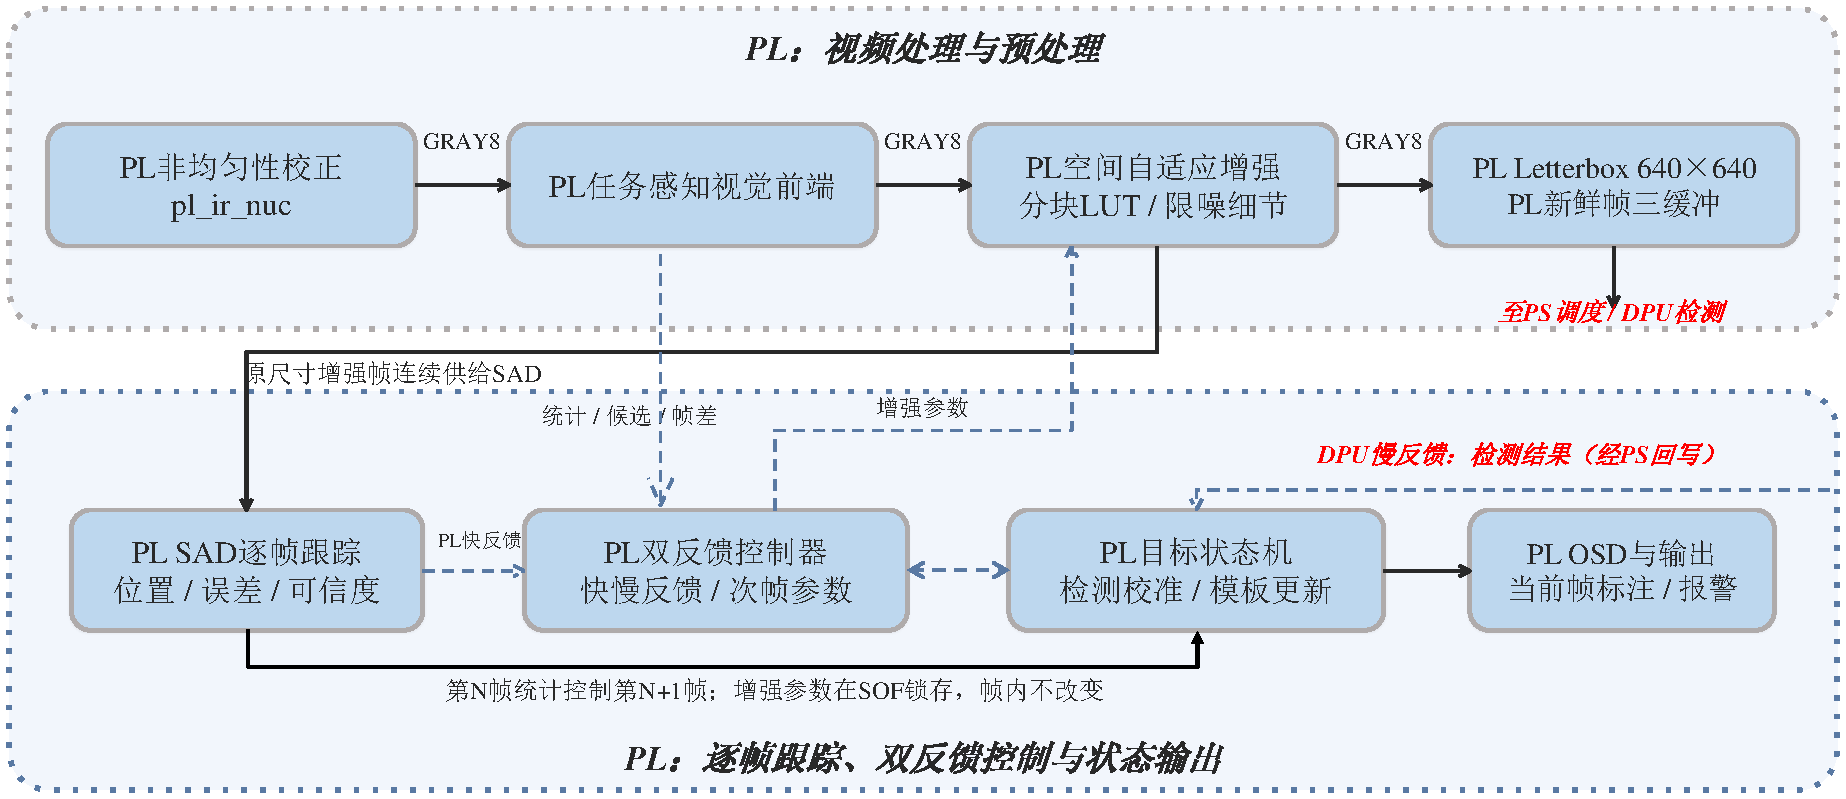
\includegraphics[width=\linewidth,height=0.58\textheight,keepaspectratio]{images/flowcharts/p04.pdf}
\caption*{图2-2 非均匀性校正、任务感知与空间自适应增强内部结构图}
\end{figure}

\paragraph*{5. 增强后图像的分流与接口关系}
空间自适应增强模块输出原尺寸增强图像后，系统根据后续任务需求将其分配至跟踪、检测和显示三个支路。分流发生在公共预处理链路之后，各支路分别完成自身所需的处理，互不替代。

\textbf{第一条为 PL 跟踪支路。} 增强后的 \(640\times480\) 原尺寸灰度图像连续送入 SAD 跟踪模块。该支路保留原始图像坐标系，用于模板匹配、目标位置更新和跟踪可信度计算，不经过检测支路的 Letterbox 变换。

\textbf{第二条为 DPU 检测支路。} 图像进入 Letterbox 模块后，按照模型输入要求进行等比例缩放和填充，生成 \(640\times640\) 的检测图像，再通过帧写入适配器和 AXI DataMover S2MM 通道写入 DDR 检测三缓冲。该支路中的像素格式、帧身份和写入状态需要保持一致，以便 PS 后续正确调用 DPU。

\textbf{第三条为视频显示支路。} 原尺寸增强图像写入独立的显示双 bank 缓存，供后续 OSD 模块叠加目标框及状态信息，并送往 HDMI 输出。显示缓存与 DPU 检测三缓冲相互独立，避免检测帧的读写占用直接影响显示图像的完整性。

三条支路共享前级增强结果，但分别维护自身的数据传输和缓存状态。特别是检测支路需要进行尺寸变换，而跟踪与显示支路保留原尺寸坐标，因此在检测结果返回后，必须依据缩放比例和填充量完成必要的坐标反变换，并结合来源 Frame ID 判断结果是否适用于当前目标状态。

通过上述分流设计，PL 能够持续完成图像预处理、逐帧跟踪和视频显示，而 DPU 只在需要时执行神经网络检测，从而形成以 PL 实时视频处理为主、DPU 间歇式推理为辅的硬件协同结构。

\paragraph*{6. 本模块关键输入输出信号}
为便于后续电路调试和模块联调，摄像头接入与 PL 视频预处理模块的主要接口关系汇总如下。

\begingroup\footnotesize\setlength{\tabcolsep}{4pt}\renewcommand{\arraystretch}{1.2}
\begin{longtable}{@{}>{\raggedright\arraybackslash}p{0.18\linewidth}>{\raggedright\arraybackslash}p{0.25\linewidth}>{\raggedright\arraybackslash}p{0.25\linewidth}>{\raggedright\arraybackslash}p{\dimexpr0.32\linewidth-24pt\relax}@{}}
\multicolumn{4}{c}{\textbf{目录表2 （1）摄像头接入与 PL 视频预处理电路接口与信号目录}}\\\toprule
接口位置 & 关键输入 & 关键输出 & 主要作用\\\midrule
\endfirsthead
\multicolumn{4}{c}{\textbf{目录表2 （1）摄像头接入与 PL 视频预处理电路接口与信号目录（续）}}\\\toprule
接口位置 & 关键输入 & 关键输出 & 主要作用\\\midrule
\endhead
\bottomrule
\endfoot
摄像头接入 & 像素数据、采样时钟、实际同步信号 & 内部像素流及同步信息 & 完成物理接口适配\\\addlinespace[3pt]
视频同步与输入检查 & \path{TDATA}、\path{TUSER}、\path{TLAST}、握手信号 & 有效像素流、有效帧状态、帧身份 & 检查图像边界并处理异常帧\\\addlinespace[3pt]
非均匀性校正 & 原始灰度像素、校正参数 & 校正后灰度像素 & 修正像素响应差异\\\addlinespace[3pt]
任务感知视觉前端 & 校正后图像 & 灰度统计、候选区域信息、帧间变化信息 & 提供场景分析依据\\\addlinespace[3pt]
双反馈控制器 & 场景分析结果、跟踪状态、DPU 检测反馈 & 增强参数、检测调度相关控制信息 & 协调增强策略与检测时机\\\addlinespace[3pt]
空间自适应增强 & 校正后图像、锁存的增强参数 & 原尺寸增强图像 & 改善灰度分布与局部细节\\\addlinespace[3pt]
图像分流接口 & 原尺寸增强图像、帧身份 & SAD 输入、检测支路输入、显示支路输入 & 向三个后续子系统提供数据\\\addlinespace[3pt]
\end{longtable}
\endgroup

综上，摄像头接入与 PL 视频预处理电路不仅完成视频数据的采集和增强，还通过统一的帧同步、参数更新和图像分流机制，为跟踪、检测和显示提供一致的数据基础。该部分的设计重点在于保证连续像素流的正确传输、增强参数的帧内一致性，以及三个后续支路之间的数据与坐标关系，为整个系统的低延迟运行奠定硬件基础。

\subsubsection*{（2）PL 逐帧跟踪与目标状态管理电路}
\paragraph*{1. SAD 匹配、模板缓存与位置计算电路}
PL 逐帧跟踪模块用于在相邻两次 DPU 目标检测之间持续更新目标位置，减少对神经网络逐帧推理的依赖。系统采用基于绝对差和（Sum of Absolute Differences，SAD）的模板匹配方法，以有效检测结果初始化跟踪模板，在后续视频帧的局部搜索区域内寻找与模板最相似的位置，并根据匹配误差判断目标位置是否可靠，从而实现红外目标的连续定位。

\begin{figure}[H]
    \centering
    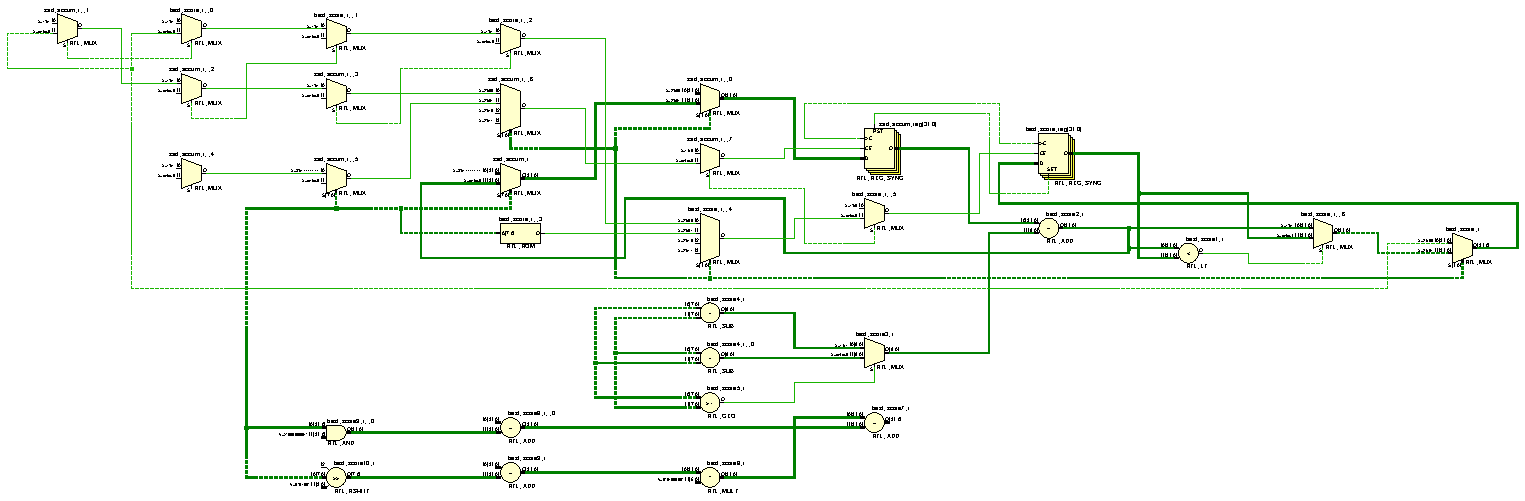
\includegraphics[width=\linewidth]{images/circuits/sad_arithmetic.pdf}
    \caption*{图2-3（a）SAD 累加与最优匹配比较电路（RTL 展开局部）}
    \vspace{6pt}
    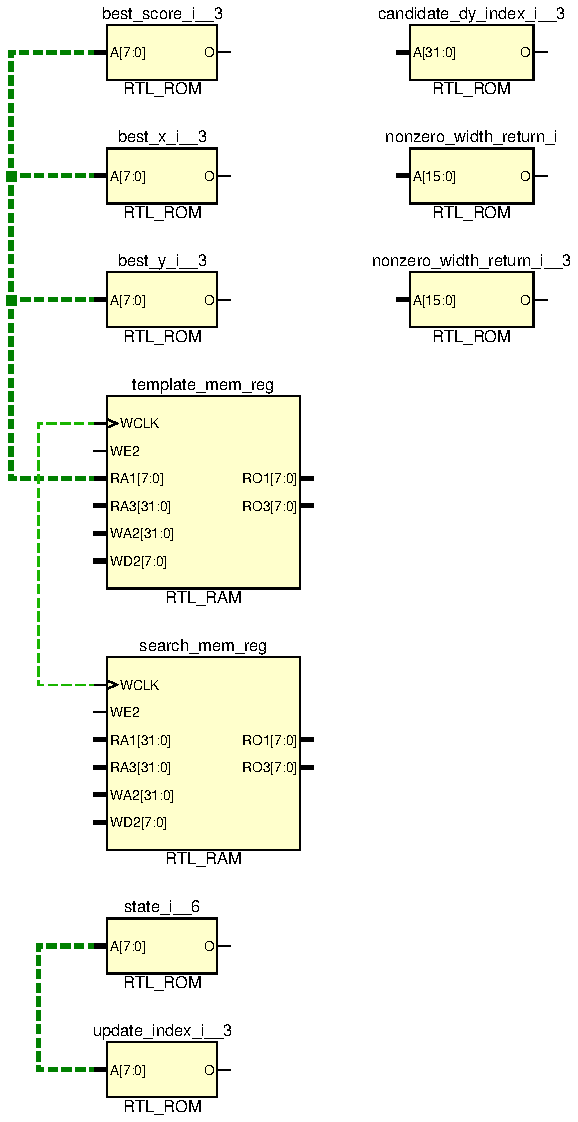
\includegraphics[height=0.38\textheight]{images/circuits/sad_memory.pdf}
    \caption*{图2-3（b）模板、搜索窗口缓存及查找逻辑（RTL 展开局部）}
\end{figure}

如图2-3所示，SAD 跟踪电路主要由模板缓存、搜索窗口生成、绝对差计算单元、并行累加单元、候选位置比较器和最优位置输出模块组成。各模块按照数据处理顺序协同工作，完成从输入图像到目标位置的硬件计算。

\subparagraph*{（1）模板初始化与缓存}
模板用于保存当前目标的局部灰度特征，是后续匹配计算的参考数据。系统在首次获得有效检测结果后，根据检测框确定目标位置，并从对应图像区域提取模板。为控制硬件资源消耗，模板不必覆盖完整检测框，而是根据目标大小选取适当的局部区域。方案中提出的候选模板尺寸为 \(16\times16\)、\(24\times24\) 和 \(32\times32\)，具体配置需要结合目标大小、纹理特征和连续跟踪实验确定。

模板数据存储在 PL 内部的块 RAM（BRAM）中，供后续各候选位置的 SAD 计算重复读取。为避免模板更新过程中出现读写冲突，系统采用双 Bank 缓存结构：一个 Bank 保存当前正在使用的模板，另一个 Bank 用于写入待更新模板。待新模板完整写入并通过有效性检查后，系统在安全的帧边界切换有效 Bank，使后续匹配统一使用新模板，避免同一次计算中混用新旧模板数据。

\subparagraph*{（2）搜索窗口生成}
每帧处理开始时，系统根据上一帧的目标位置和运动变化情况，确定当前帧的搜索中心。为减小目标运动导致的搜索区域偏移，可以利用连续两帧的目标位置估计运动方向，并采用带限幅的常速度预测确定当前帧的搜索中心。

设上一帧目标中心为 \((x_{t-1},y_{t-1})\)，再前一帧目标中心为 \((x_{t-2},y_{t-2})\)，则一种简单的运动预测方式为：

\[
\begin{aligned}
\Delta x_t &= x_{t-1}-x_{t-2},\\
\Delta y_t &= y_{t-1}-y_{t-2},\\
\hat{x}_t &= x_{t-1}
+\operatorname{clip}(\Delta x_t,-d_{\max},d_{\max}),\\
\hat{y}_t &= y_{t-1}
+\operatorname{clip}(\Delta y_t,-d_{\max},d_{\max}).
\end{aligned}
\]

其中，\((\hat{x}_t,\hat{y}_t)\) 为预测位置，\(d_{\max}\) 为单帧预测位移的限幅参数。该预测仅用于确定搜索中心，不直接作为最终跟踪结果。

以预测位置为中心，硬件生成局部搜索窗口，对其中多个候选位置进行模板匹配。方案提出的候选搜索半径包括 \(\pm8\) 和 \(\pm16\) 像素，并可根据目标运动幅度与跟踪不确定度选择搜索范围。搜索半径过小，可能无法覆盖快速移动的目标；搜索半径过大，则会增加候选位置数量和匹配计算量。因此，需要在目标运动范围、硬件资源和处理延迟之间进行权衡。

当目标位置接近搜索窗口边缘，或者连续帧的匹配误差增大时，系统应降低对当前跟踪结果的信任程度，并根据目标状态管理策略扩大搜索范围或触发重新检测。

\subparagraph*{（3）SAD 匹配计算}
确定搜索窗口后，SAD 计算模块逐一比较模板与候选图像区域之间的灰度差异。设模板为 \(T(i,j)\)，当前图像为 \(I(x,y)\)，模板尺寸为 \(W\times H\)，候选位置为 \((u,v)\)，则该位置的 SAD 值定义为：

\[
\operatorname{SAD}(u,v)=
\sum_{i=0}^{W-1}
\sum_{j=0}^{H-1}
\left|I(u+i,v+j)-T(i,j)\right|.
\]

SAD 值反映候选区域与模板之间的累计灰度差异。通常情况下，SAD 值越小，说明候选区域与模板越相似。对搜索窗口内所有候选位置完成计算后，系统选择 SAD 最小的位置作为当前帧的最佳匹配位置：

\[
(u^*,v^*)=
\underset{(u,v)\in\Omega_t}{\arg\min}
\operatorname{SAD}(u,v),
\]

其中，\(\Omega_t\) 表示当前帧的搜索窗口。

在硬件实现上，绝对差计算单元负责计算对应像素之间的差值并取绝对值，累加单元负责将多个像素差异求和，候选位置比较器负责比较不同候选位置的 SAD 值，最小值归约器最终输出最佳匹配位置及对应误差。

为提高处理吞吐率，可根据资源和时序条件采用 4 或 8 个像素并行处理，并结合模板 BRAM 和搜索区域数据复用减少重复访存。具体并行度需要结合 FPGA 资源占用、时钟频率和目标帧率要求确定。

当最佳匹配位置确定后，系统将其转换为当前目标的位置坐标，并结合模板尺寸得到跟踪框。由于 SAD 仅比较灰度差异，外观相似的背景区域也可能获得较小的匹配误差，因此不能仅凭最小 SAD 值就认定跟踪成功，还需要进一步计算跟踪可信度。

\subparagraph*{（4）跟踪可信度计算}
为了判断当前匹配结果是否可靠，系统综合考虑匹配误差和最佳匹配位置的唯一性。方案提出的归一化误差指标为：

\[
E=\frac{\operatorname{SAD}_{\min}}{W H\cdot255},
\]

其中，\(\operatorname{SAD}_{\min}\) 为当前搜索窗口内的最小 SAD 值。对于 8 位灰度图像，单个像素的最大灰度差为 255，因此该指标可以衡量归一化后的平均灰度差异。一般而言，\(E\) 越小，说明模板与最佳匹配区域越接近。

此外，系统通过比较最佳匹配值与次优匹配值，判断当前最优位置是否具有足够的区分度。设排除最佳位置附近抑制区域后得到的次优匹配值为 \(\operatorname{SAD}_{\mathrm{second}}\)，则可定义：

\[
R=
\frac{\operatorname{SAD}_{\mathrm{second}}-
\operatorname{SAD}_{\min}}
{\operatorname{SAD}_{\mathrm{second}}+\varepsilon},
\]

其中，\(\varepsilon\) 为防止分母为零的微小正数。\(R\) 越大，说明最佳匹配位置相对于其他候选位置越突出；\(R\) 越小，则可能存在多个相似区域，目标位置的不确定性更高。计算次优匹配值时，需要排除最佳位置附近的抑制窗口，避免相邻的高度相关位置影响判断。

系统将归一化误差、匹配唯一性、目标位置连续性和搜索窗口边界状态共同作为跟踪可信度判断依据。当匹配误差较小、最优位置具有较高区分度且目标运动连续时，可以认为当前匹配结果相对可靠；当误差增大、最佳位置不突出，或者目标持续出现在搜索窗口边缘时，则应降低对该结果的信任程度。

具体阈值需要通过连续红外视频实验确定。在硬件版本冻结前，还应在软件参考实现中比较原始 SAD、均值归一化 SAD 和梯度 SAD 等方案，评估红外图像整体亮度变化对匹配稳定性的影响。

\paragraph*{2. 目标状态机、检测结果校正及反馈控制}
SAD 模块负责逐帧计算目标位置，但它不能独立解决目标丢失、长期漂移和模板污染等问题。因此，系统在 PL 端设置目标状态管理模块，将 SAD 匹配结果、跟踪可信度和目标检测结果统一纳入状态机控制，实现目标初始化、连续跟踪、异常处理、位置校正和模板更新。

\begin{figure}[H]\centering
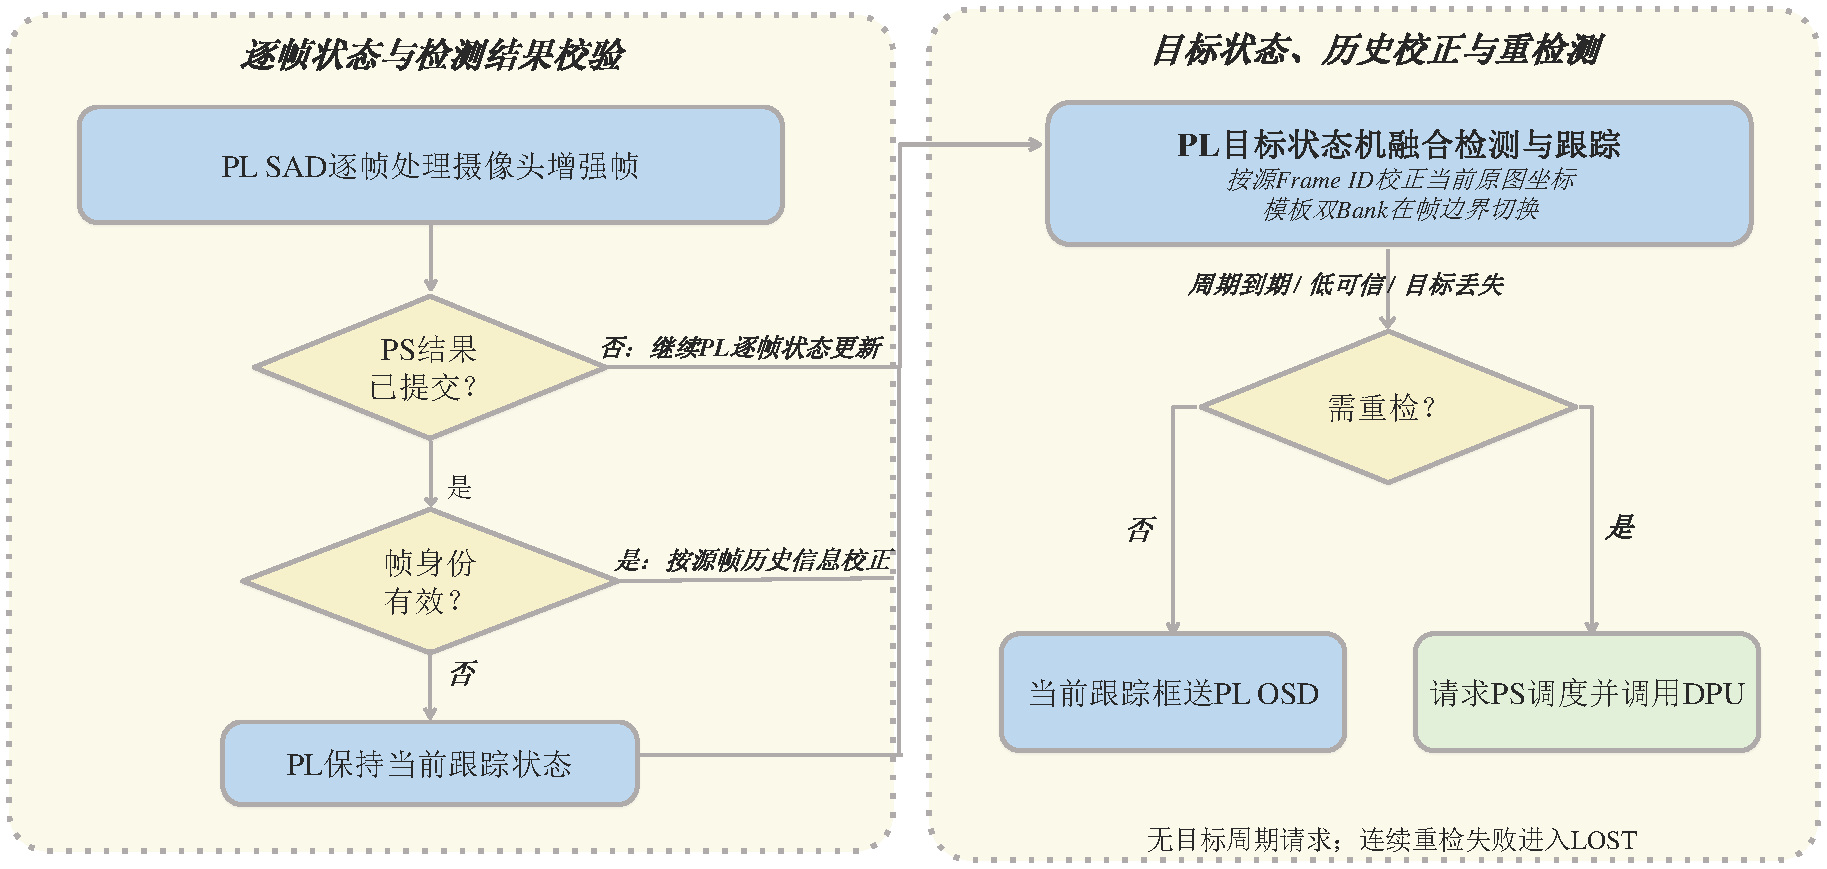
\includegraphics[width=\linewidth,height=0.58\textheight,keepaspectratio]{images/flowcharts/p11.pdf}
\caption*{图2-4 目标状态机、检测结果校正及反馈接口图}
\end{figure}

图2-4应展示 SAD 模块、目标状态机、模板缓存和检测结果之间的关系。其中，SAD 模块持续提供当前帧的匹配位置与可信度，目标状态机根据跟踪状态和检测反馈决定是否修正目标位置、更新模板或重新检测，从而形成连续定位与周期纠偏相结合的控制机制。

\subparagraph*{（1）目标状态机与状态转换}
目标状态机用于管理目标从尚未发现到初始化、连续跟踪、重新检测和丢失恢复的完整过程。系统可划分为以下状态：

- \textbf{WAIT\_TARGET：} 当前尚未获得有效目标，等待检测结果。

- \textbf{DPU\_DETECT：} 系统正在执行初始检测，等待有效检测结果。

- \textbf{INIT\_TEMPLATE：} 根据有效检测框初始化模板缓存和目标位置。

- \textbf{PL\_TRACK：} 由 PL 逐帧执行 SAD 匹配，更新目标位置并计算可信度。

- \textbf{REDETECT：} 达到周期检测条件或跟踪可信度下降时，等待重新检测结果。

- \textbf{LOST：} 连续检测失败或目标无法可靠定位时，将目标标记为丢失，等待后续检测恢复。

正常情况下，系统在首次检测成功后进入模板初始化状态，随后进入 PL 跟踪状态。跟踪可信度满足要求时，系统继续逐帧更新位置；当达到预设检测周期，或出现低可信度、目标接近搜索边界等情况时，状态机触发重新检测。

如果重新检测成功，系统利用返回的检测框校正目标位置，并根据检测结果和跟踪可信度决定是否重新初始化或更新模板，再恢复逐帧跟踪。如果连续多次检测仍未找到目标，则进入丢失状态，停止将不可靠的匹配结果作为有效目标位置，并等待后续检测恢复。

为防止单帧噪声造成状态频繁切换，低可信状态、模板更新和丢失判定应采用连续多帧确认或滞回机制。检测周期 \(K\)、可信度阈值和连续失败次数均需要通过实验确定，不宜在缺乏实测数据时直接宣称为最优配置。

\subparagraph*{（2）检测结果校正与历史状态关联}
PL 逐帧跟踪与 DPU 检测并行工作。由于 DPU 检测结果存在推理和后处理延迟，返回的检测框可能对应此前已经处理过的视频帧。因此，PL 不能直接将检测框覆盖当前跟踪位置，而应结合检测结果对应的帧编号及历史跟踪记录进行校正。

系统为已处理帧保留必要的历史跟踪信息，包括目标框、运动状态及相关时间信息。当检测结果返回后，PL 根据其来源帧编号找到对应的历史跟踪记录，并比较该帧的检测框与历史跟踪框之间的位置偏差。在检测结果有效且可信的前提下，系统结合当前跟踪状态，对当前目标位置进行有界修正。

例如，DPU 返回的是第 \(N\) 帧的检测结果，而当前视频已经处理到第 \(M\) 帧，且 \(M>N\)。系统先比较第 \(N\) 帧的检测框与第 \(N\) 帧历史跟踪框之间的差异，再结合当前跟踪状态和运动变化，对第 \(M\) 帧的目标位置进行有限修正。这样可以利用检测结果纠正跟踪漂移，同时避免将历史坐标直接用于当前画面。

为避免异常检测结果破坏正常跟踪，校正量需要进行限幅，并根据检测置信度、结果帧龄和当前跟踪可信度进行判断。如果检测结果与当前跟踪状态明显冲突，或者来源帧与历史记录不匹配，则不应直接更新当前目标位置，而应交由状态机进一步处理。

\subparagraph*{（3）重检测触发与状态反馈}
系统采用周期检测与事件触发相结合的策略。周期检测用于定期校正长期跟踪误差；事件触发则用于处理目标快速运动、匹配可信度下降和目标疑似丢失等情况。

主要触发条件包括：

1. 尚未发现有效目标，需要执行初始检测；

2. 距离上一次有效检测已达到预设帧间隔 \(K\)；

3. SAD 归一化误差持续超过阈值，或最佳匹配位置的唯一性不足；

4. 目标位置接近搜索窗口边缘，现有搜索范围可能无法覆盖目标；

5. 场景变化明显，现有跟踪结果可能不再可靠；

6. 当前跟踪结果进入丢失状态，需要尝试重新获取目标。

当有效触发条件成立时，PL 状态机产生重新检测请求。系统在等待检测结果期间仍然继续处理后续视频帧，并根据 SAD 结果更新当前目标位置。检测完成后，返回结果由状态机进行有效性判断，并决定是否修正位置、更新模板或进入目标丢失状态。

通过上述机制，PL 负责连续定位和重检测决策，DPU 负责按需提供检测结果，二者形成互补，而不是让视频处理链路等待每次神经网络推理完成。

\subparagraph*{（4）模板更新与目标丢失恢复}
模板更新直接影响 SAD 跟踪的长期稳定性。如果目标外观发生缓慢变化，而模板始终保持不变，匹配误差可能逐渐增大；但如果在低可信度时仍然无条件更新模板，则可能把背景区域写入模板，导致目标漂移持续累积。

因此，系统采用有条件的模板更新策略：

- 首次检测成功后，根据有效目标框初始化模板；

- 周期重检测或事件触发检测成功后，结合检测结果和当前状态更新目标位置及模板；

- PL 逐帧跟踪可信度较高时，可根据实验确定的更新策略缓慢调整模板，以适应目标外观的渐进变化；

- PL 逐帧跟踪可信度较低时，禁止仅根据当前 SAD 结果直接更新模板，避免将背景写入模板。

模板更新采用双 Bank 缓存：跟踪期间由当前有效 Bank 提供模板数据，待更新模板写入另一 Bank；待模板完整写入并通过检查后，再在安全帧边界切换有效 Bank。这样可以避免模板读写冲突，并保证一次匹配计算始终使用完整、一致的模板数据。

当目标连续多帧无法可靠匹配时，状态机进入丢失状态，禁止继续输出未经确认的低可信位置。系统随后重新检测目标；若检测成功，则根据返回的检测框重新初始化目标位置与模板，恢复 PL 逐帧跟踪；若连续检测失败，则继续保持目标丢失状态，等待后续检测，而不将不可靠结果当作有效定位输出。

\paragraph*{3. 本模块关键输入输出信号}
为明确 SAD 运算、目标状态管理与模板更新之间的接口关系，主要输入输出信号汇总如下。

\begingroup\footnotesize\setlength{\tabcolsep}{4pt}\renewcommand{\arraystretch}{1.2}
\begin{longtable}{@{}>{\raggedright\arraybackslash}p{0.18\linewidth}>{\raggedright\arraybackslash}p{0.25\linewidth}>{\raggedright\arraybackslash}p{0.25\linewidth}>{\raggedright\arraybackslash}p{\dimexpr0.32\linewidth-24pt\relax}@{}}
\multicolumn{4}{c}{\textbf{目录表3 （2）PL 逐帧跟踪与目标状态管理电路接口与信号目录}}\\\toprule
模块 & 关键输入 & 关键输出 & 主要作用\\\midrule
\endfirsthead
\multicolumn{4}{c}{\textbf{目录表3 （2）PL 逐帧跟踪与目标状态管理电路接口与信号目录（续）}}\\\toprule
模块 & 关键输入 & 关键输出 & 主要作用\\\midrule
\endhead
\bottomrule
\endfoot
模板缓存 & 初始化目标区域、模板更新控制 & 当前有效模板、模板版本 & 保存并安全更新跟踪模板\\\addlinespace[3pt]
搜索窗口生成 & 历史目标位置、运动变化、跟踪不确定度 & 搜索中心、搜索范围 & 限定候选匹配区域\\\addlinespace[3pt]
SAD 匹配计算 & 当前图像、模板、搜索窗口 & 最小 SAD、次优 SAD、最佳位置 & 计算候选区域的匹配程度\\\addlinespace[3pt]
可信度计算 & 匹配误差、匹配唯一性、位置连续性 & 可信度、异常标志 & 判断当前跟踪结果是否可靠\\\addlinespace[3pt]
目标状态机 & 跟踪位置、可信度、检测校正结果 & 当前目标状态、位置更新控制 & 管理初始化、跟踪、重检测与丢失恢复\\\addlinespace[3pt]
模板更新控制 & 目标状态、跟踪可信度、有效检测结果 & 模板更新允许信号、Bank 切换控制 & 防止错误模板更新\\\addlinespace[3pt]
\end{longtable}
\endgroup

综上，PL 逐帧跟踪与目标状态管理电路以 SAD 模板匹配为基础，通过搜索窗口限制计算范围，利用归一化误差和匹配唯一性判断跟踪可信度，再由目标状态机协调连续跟踪、检测结果校正、模板更新和目标丢失恢复。PL 在相邻检测时刻之间持续承担目标定位任务，DPU 则在周期到达或跟踪异常时提供检测结果。通过双 Bank 模板缓存、有条件的模板更新和历史状态校正，系统能够降低低可信匹配引起的持续漂移风险，并避免延迟检测结果直接覆盖当前目标位置，为后续视频显示和低延迟目标定位提供可靠的硬件基础。

\subsubsection*{（3）DPU 检测数据通路与 PS—PL 控制接口电路}

\begin{figure}[H]\centering
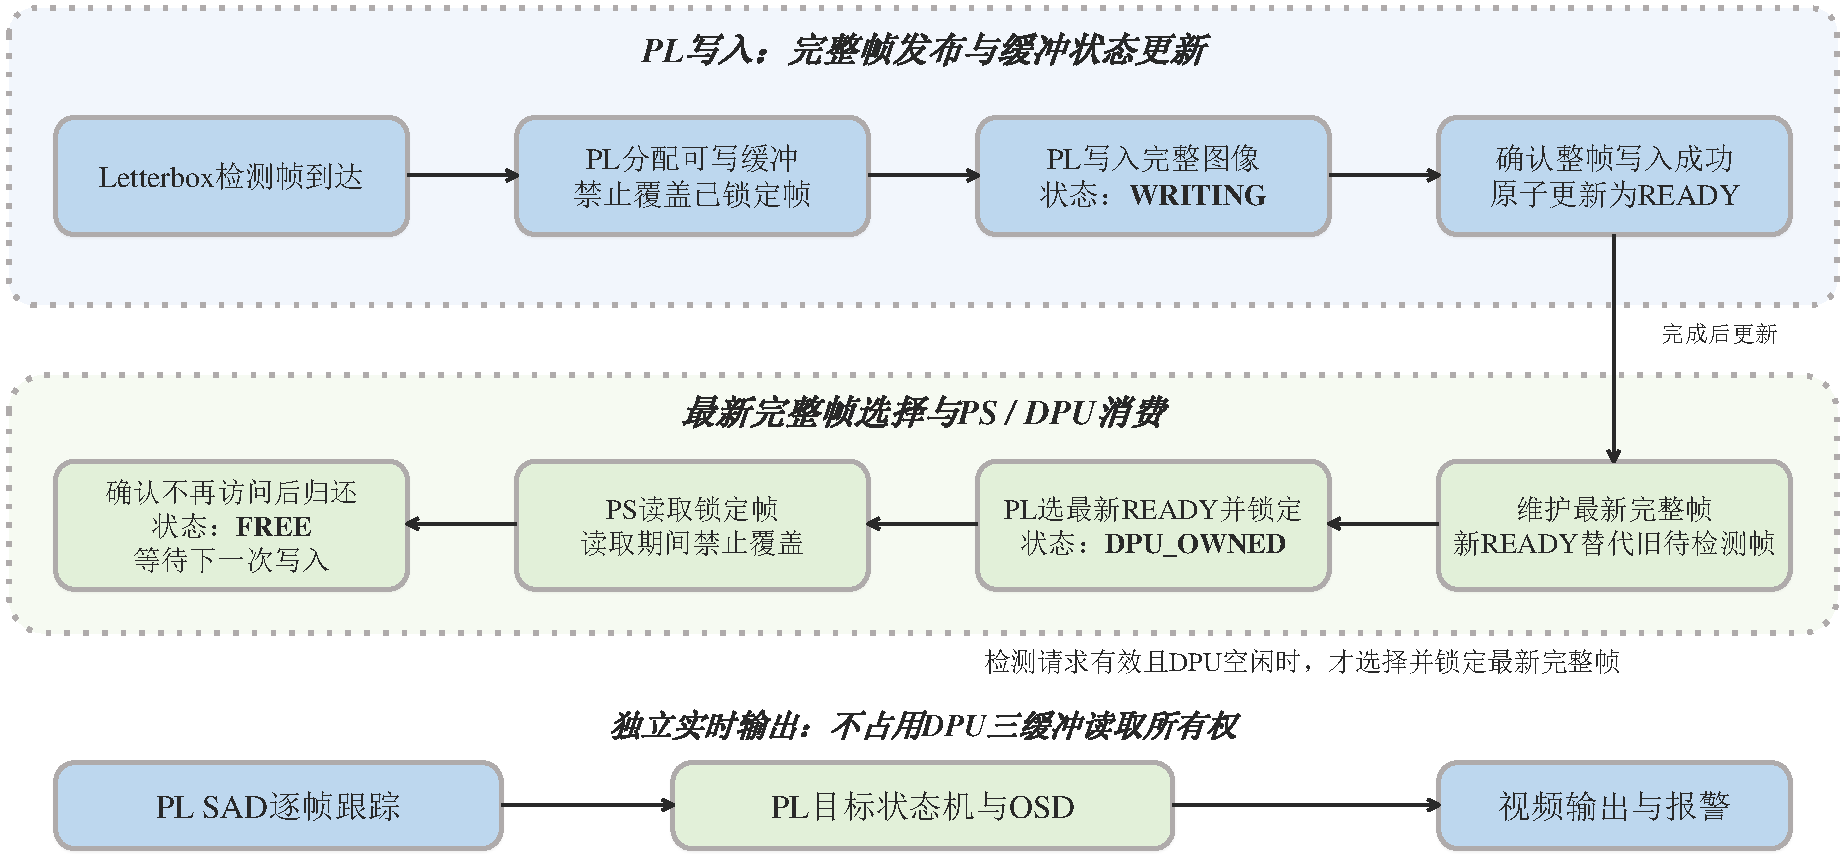
\includegraphics[width=\linewidth,height=0.58\textheight,keepaspectratio]{images/flowcharts/p06.pdf}
\caption*{图2-5 Letterbox、DDR 三缓冲帧池与 DPU 检测数据通路图}
\end{figure}

\paragraph*{1. DPU 检测数据通路总体结构}
DPU 检测数据通路负责将 PL 端生成的检测图像提供给 PS 端，由 PS 调用 YOLOv8n INT8 模型执行目标检测，并将检测结果返回 PL。该部分主要包括 Letterbox 图像预处理、DPU 专用三缓冲帧池、PS 端检测调度、DPU 推理、检测结果后处理以及 PS—PL 控制接口。


如图2-5所示，经过 PL 端图像预处理后的原尺寸红外图像分为跟踪、检测和显示支路。其中，检测支路通过 Letterbox 模块完成尺寸调整和边缘填充，形成符合模型输入尺寸要求的检测图像。检测图像进入 DPU 专用三缓冲帧池，并由帧调度逻辑记录完整帧的编号、缓冲区状态及相关信息。

当 PL 产生检测请求时，PS 获取请求信息，并依据缓冲区状态选择最新的完整检测帧。随后，PS 根据模型实际输入要求准备输入张量，调用 VART 等运行时接口执行 YOLOv8n INT8 模型推理。

推理完成后，PS 对网络输出进行解码、置信度筛选、非极大值抑制（NMS）及坐标还原，得到目标框和置信度等检测信息。检测结果通过 PS—PL 控制接口返回 PL，并携带对应的来源 Frame ID，以便后续目标状态管理逻辑判断该结果的有效性。

该数据通路采用间歇式检测机制。PL 持续承担视频处理与逐帧跟踪任务，DPU 根据预设检测周期或跟踪异常请求执行推理，从而减少逐帧神经网络推理带来的等待开销。

\paragraph*{2. 检测图像预处理与缓冲区管理}
\subparagraph*{（1）Letterbox 图像尺寸变换}
Letterbox 模块负责将原尺寸红外图像转换为 YOLOv8n 模型要求的固定输入尺寸。该模块保持原图宽高比进行缩放，再通过边缘填充补齐剩余区域，避免直接拉伸图像造成目标形状变化。

本系统原图尺寸为 \(640\times480\)，模型输入尺寸为 \(640\times640\)，缩放比例为：

\[
r=\min\left(\frac{640}{640},\frac{640}{480}\right)=1.
\]

因此，图像保持原尺寸，上下两侧各填充 80 行像素，得到 \(640\times640\) 的检测图像，填充值为 114。

红外图像采用单通道灰度格式时，将同一灰度值复制到 R、G、B 三个颜色通道，形成 RGB888 图像。随后，根据实际部署模型的输入要求，由 PS 端完成必要的归一化、量化及张量格式组织。

Letterbox 仅用于检测支路。PL 逐帧跟踪和视频显示继续使用原尺寸图像，避免检测图像的补边操作影响跟踪与显示所使用的原图坐标。

\subparagraph*{（2）DPU 专用三缓冲帧池}
由于视频输入持续进行，而 DPU 推理需要一定时间，输入帧率与检测处理速率之间可能存在差异。如果所有待检测图像均按照先进先出的顺序排队，DPU 就可能持续处理已经过时的图像，使检测结果无法及时反映当前场景。

为此，系统采用 DPU 专用三缓冲帧池，并通过 Fresh-Frame 策略优先选择最新的完整帧。

三个缓冲区根据数据生命周期承担不同作用：

- \textbf{WRITE\_BUFFER：} 接收当前正在写入的检测帧。

- \textbf{LATEST\_READY\_BUFFER：} 保存最新的完整有效帧，等待检测调度。

- \textbf{READ\_BUFFER：} 保存已交由 DPU 读取或正在参与推理的帧。

每个缓冲区关联相应的状态、Frame ID、时间戳、所有权和复用代次。缓冲区状态包括 \path{FREE}、\path{WRITING}、\path{READY} 和 \path{DPU_OWNED}。

当一帧完成写入并确认有效后，缓冲区才能从 \path{WRITING} 转为 \path{READY}。PS 选择该帧执行检测后，将其标记为 \path{DPU_OWNED}，在 DPU 不再使用该缓冲区之前，不允许输入端覆盖其中的数据。

当新的完整帧到达时，如果存在尚未被 DPU 读取的旧帧，调度逻辑可以将其标记为过期帧，优先保留最新有效帧。若没有可用的写入缓冲区，则按照缓冲区管理策略处理输入压力，并记录相应的异常或丢帧信息。

需要注意，输入帧完成与缓冲区写入完成是两个不同事件。只有确认整帧数据完整有效，才能将其发布给检测调度程序。三缓冲机制只服务于 DPU 检测数据通路，不作为 HDMI 显示缓存使用。

\paragraph*{3. PS 端检测调度与 DPU 推理}
\subparagraph*{（1）检测请求与最新帧选择}
PS 端运行于 Zynq UltraScale+ MPSoC 的处理系统中，负责检测任务调度、模型调用及检测结果后处理。

当 PL 产生新的检测请求时，PS 获取请求序号、来源帧编号、缓冲区编号和请求原因等信息，并检查是否存在可用的完整检测帧。

系统采用请求序号机制识别新的检测任务。PS 将当前请求序号与上一次处理的序号进行比较，以判断是否出现新的检测请求，避免仅依赖短时脉冲而遗漏请求。

在多个完整帧可供选择时，PS 优先获取最新的有效帧，而不是依次处理所有历史图像。选定缓冲区后，需要保证其数据在推理期间保持有效，避免输入端覆盖仍在使用的图像。

检测请求可以由以下情况触发：

1. 尚未发现目标，需要执行初始检测。

2. 达到预设的周期重检测间隔。

3. PL 跟踪可信度下降。

4. 目标丢失或跟踪状态异常。

通过上述机制，DPU 仅在需要时执行检测，而不必对每一帧视频重复运行完整神经网络。

\subparagraph*{（2）模型输入准备与 DPU 调用}
PS 获取完整检测帧后，按照模型实际要求准备输入张量，并调用部署在 DPU 上的 YOLOv8n INT8 模型。

输入准备过程包括读取检测图像、确认颜色通道顺序、完成必要的归一化和量化，以及按照实际运行时要求组织张量。具体数据布局和量化参数以最终部署模型及 VART Runner 的输入张量信息为准。

本系统使用经过硬件适配、INT8 量化并编译的 YOLOv8n 模型，目标 DPU 架构为 \path{DPUCZDX8G_ISA1_B4096}。实际运行时需要保证加载的 Overlay 与编译后的 XModel 相匹配。

DPU 完成推理后，PS 获取模型输出，并进入检测结果后处理流程。推理期间，PL 继续处理后续视频帧，完成逐帧跟踪与视频输出，不需要等待 DPU 返回结果后才能继续工作。

\subparagraph*{（3）检测结果后处理}
DPU 输出的是网络预测张量，需要由 PS 进一步解析，才能获得可供 PL 使用的目标检测结果。

PS 根据模型实际输出结构完成候选框解码，并根据置信度阈值筛除低可信度候选框。随后执行非极大值抑制，减少多个高度重叠的候选框对同一目标的重复检测。

当前方案采用单类别 \path{tank} 检测模型，后处理结果包括目标框位置、类别和置信度等信息。具体解码方式、阈值和 NMS 参数应与实际部署模型的输出结构保持一致。

处理完成后，PS 将目标框坐标从模型输入坐标系还原到原始图像坐标系。

\subparagraph*{（4）检测框坐标还原}
由于检测图像经过 Letterbox 处理，网络输出坐标对应 \(640\times640\) 的模型输入图像，而原图尺寸为 \(640\times480\)，因此需要去除补边偏移。

设模型输出框左上角坐标为 \((x_m,y_m)\)，缩放比例为 \(r\)，左侧和顶部填充值分别为 \(p_x\) 和 \(p_y\)，则原图坐标为：

\[
x_o=\frac{x_m-p_x}{r},\qquad
y_o=\frac{y_m-p_y}{r}.
\]

对于右下角坐标 \((x'_m,y'_m)\)，则有：

\[
x'_o=\frac{x'_m-p_x}{r},\qquad
y'_o=\frac{y'_m-p_y}{r}.
\]

本系统采用 \(640\times480\) 原图和 \(640\times640\) 检测输入，上下各填充 80 行，因此 \(r=1\)、\(p_x=0\)、\(p_y=80\)。恢复原图坐标时，纵坐标需要减去 80。

完成坐标还原后，还需要将检测框限制在原图有效范围内，检查框的位置、宽度和高度是否合理。

最终，PS 将检测框、置信度、来源 Frame ID 以及相关缓冲区身份信息组织为完整结果，通过控制接口提交给 PL。

\paragraph*{4. PS—PL 控制接口与检测结果回传}
\begin{figure}[H]\centering
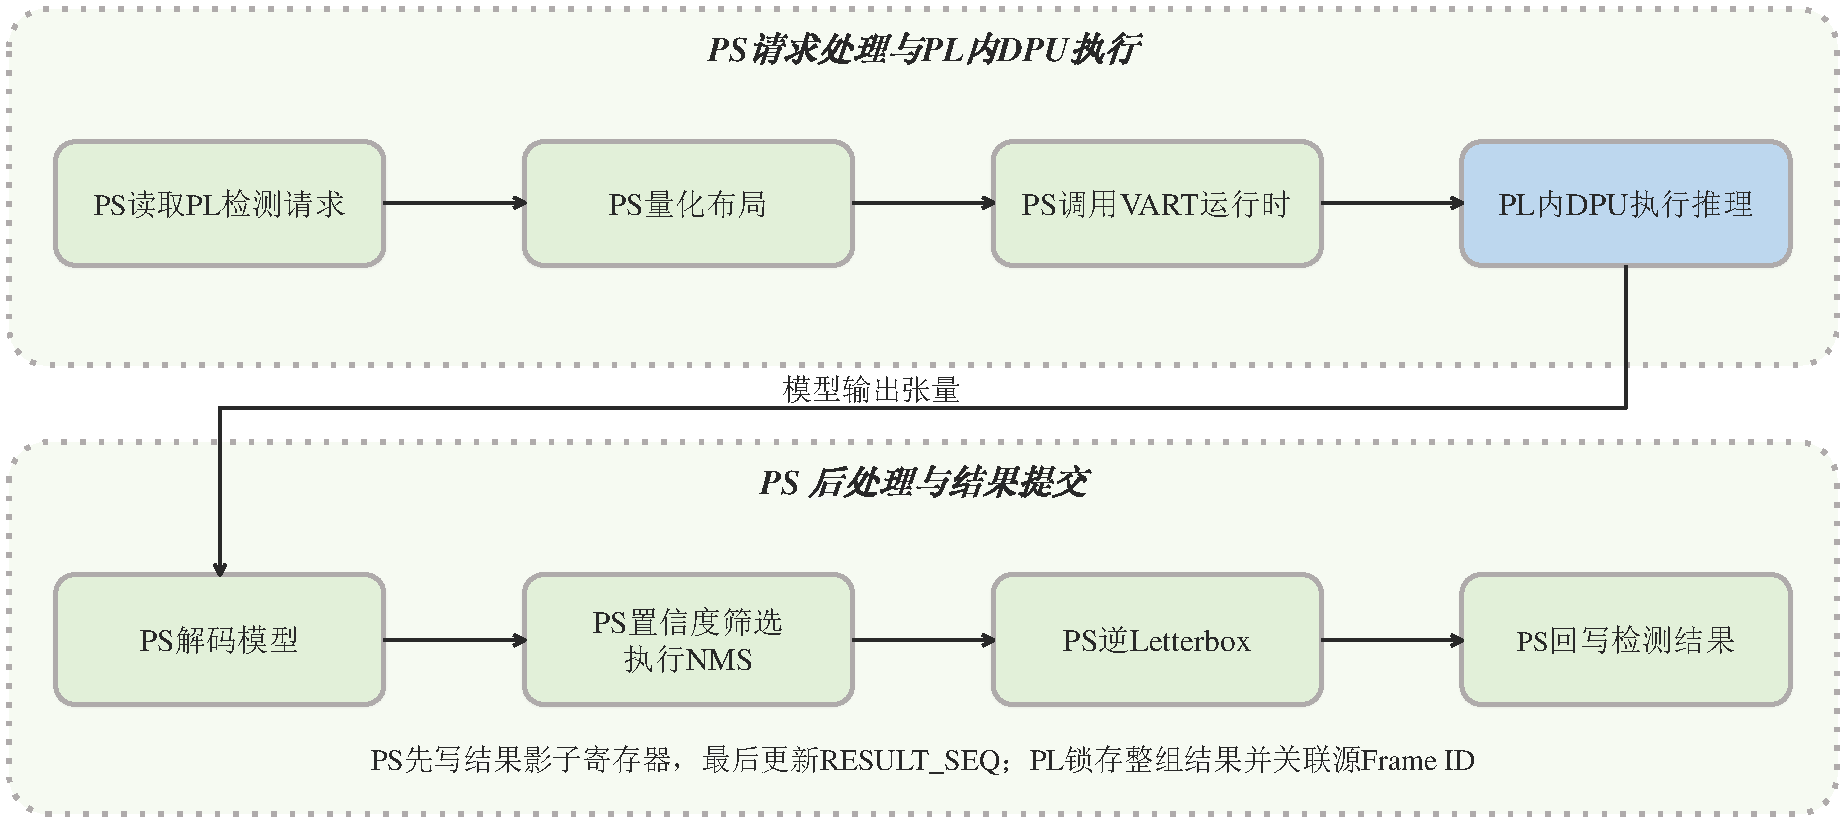
\includegraphics[width=\linewidth,height=0.58\textheight,keepaspectratio]{images/flowcharts/p10.pdf}
\caption*{图2-6 PS—PL 检测请求、DPU 推理与结果回传接口图}
\end{figure}

PS 与 PL 之间通过 AXI4-Lite 控制接口交换检测请求、运行状态和检测结果。图像数据与控制信息分别通过各自的通路处理：检测图像由 DPU 专用帧池提供，AXI4-Lite 则负责传递任务状态和检测结果等信息。

\subparagraph*{（1）控制寄存器与状态信息}
根据《烽眼》方案，PS—PL 控制接口的寄存器规划如下。

可参照本节末“电路接口与信号表格目录”的目录表4（（3）DPU 检测数据通路与 PS—PL 控制接口电路接口与信号目录）。

以上地址和字段按照《烽眼》方案中的寄存器规划列出，实际使用时以最终 RTL 寄存器定义为准。

\subparagraph*{（2）检测请求握手}
当 PL 需要执行目标检测时，更新 \path{REQUEST_SEQ}，并记录相应的来源帧编号、缓冲区编号及请求原因。

PS 读取请求序号后，与上一次处理的序号进行比较。若序号发生变化，则表明存在新的检测任务，PS 随后读取对应的请求信息，获取最新有效检测帧并调用 DPU。

采用序号握手可以避免短时请求脉冲在 PS 忙于其他任务时被遗漏。请求序号与相关帧身份信息应保持对应，保证 PS 调用 DPU 时能够确定实际处理的是哪一帧图像。

\subparagraph*{（3）检测结果提交}
一次检测结果包含来源帧编号、检测框坐标、宽高及置信度等多个字段。如果 PL 在 PS 尚未写完所有字段时读取数据，就可能将新旧结果混合使用。

为此，系统采用结果提交序号机制。PS 首先写入完整检测结果的各项字段，最后更新 \path{RESULT_SEQ}，表示一组完整结果已经提交。

PL 检测到新的结果序号后，才锁存整组结果，并检查来源帧编号及结果有效性。这样可以保证检测框坐标、置信度和来源帧身份属于同一次推理任务。

检测完成但未发现目标时，也应通过明确的状态信息区分无有效目标、检测未完成和检测异常，避免将无目标结果误认为旧目标仍然有效。

\subparagraph*{（4）Frame ID 与缓冲区身份关联}
PS 提交检测结果时，必须保留 DPU 实际处理的来源 Frame ID，不能直接使用当前最新帧的编号替代。

例如，DPU 处理的是 Frame 100，即使推理完成前 PL 已经处理到 Frame 105，返回的检测结果仍然属于 Frame 100。PL 需要根据来源帧编号判断结果的时间关系，再结合历史跟踪状态进行校正，而不是直接将历史检测框作为 Frame 105 的当前位置。

同时，缓冲区编号和复用代次用于识别检测任务所使用的帧池资源。只有来源帧编号、缓冲区编号和复用代次等身份信息符合预期时，才允许释放相应的缓冲区，避免迟到的检测结果误释放已经被重新使用的缓冲区。

通过统一管理请求序号、结果序号、Frame ID 和缓冲区身份，系统能够保证图像输入、DPU 推理及检测结果回传之间的关联关系。

\paragraph*{5. 关键输入输出与接口关系}
\begingroup\footnotesize\setlength{\tabcolsep}{4pt}\renewcommand{\arraystretch}{1.2}
\begin{longtable}{@{}>{\raggedright\arraybackslash}p{0.18\linewidth}>{\raggedright\arraybackslash}p{0.25\linewidth}>{\raggedright\arraybackslash}p{0.25\linewidth}>{\raggedright\arraybackslash}p{\dimexpr0.32\linewidth-24pt\relax}@{}}
\multicolumn{4}{c}{\textbf{目录表5 （3）DPU 检测数据通路与 PS—PL 控制接口电路接口与信号目录}}\\\toprule
模块 & 主要输入 & 主要输出 & 功能\\\midrule
\endfirsthead
\multicolumn{4}{c}{\textbf{目录表5 （3）DPU 检测数据通路与 PS—PL 控制接口电路接口与信号目录（续）}}\\\toprule
模块 & 主要输入 & 主要输出 & 功能\\\midrule
\endhead
\bottomrule
\endfoot
Letterbox & 原尺寸增强图像 & 固定尺寸检测图像 & 保持宽高比并完成边缘填充\\\addlinespace[3pt]
DPU 专用三缓冲帧池 & 检测图像、帧身份和缓冲状态 & 最新完整帧及其身份信息 & 管理检测帧生命周期\\\addlinespace[3pt]
PS 检测调度 & 检测请求、帧身份和缓冲状态 & 检测任务及 DPU 调用 & 选择最新有效帧\\\addlinespace[3pt]
DPU 推理 & 满足模型要求的输入张量 & 网络预测结果 & 执行 YOLOv8n INT8 推理\\\addlinespace[3pt]
检测结果后处理 & 网络输出张量 & 检测框、置信度及类别 & 完成解码、筛选、NMS 和坐标还原\\\addlinespace[3pt]
AXI4-Lite 控制接口 & 检测请求、状态和结果字段 & 请求状态及完整检测结果 & 完成 PS—PL 控制信息交换\\\addlinespace[3pt]
缓冲区与异常管理 & 缓冲状态、结果身份及错误状态 & 缓冲区释放、丢帧统计和错误信息 & 保证资源使用和结果关联正确\\\addlinespace[3pt]
\end{longtable}
\endgroup

综上，DPU 检测数据通路与 PS—PL 控制接口围绕检测帧管理、间歇式 DPU 推理和检测结果回传展开。系统通过 DPU 专用三缓冲及 Fresh-Frame 机制减少过期帧积压，通过 AXI4-Lite 请求与结果序号保证软硬件控制信息的完整传递，并利用 Frame ID 和缓冲区身份关联检测结果与原始图像。该设计使 PL 能够持续执行视频处理与逐帧跟踪，而 DPU 按照检测需求提供目标校正信息。

\subsubsection*{（4）视频显示输出与时序接口电路}
\paragraph*{1. 视频显示输出总体结构}
视频显示输出电路负责将 PL 端处理后的红外图像与当前有效的目标位置、跟踪状态等信息进行整合，生成符合 HDMI 输出要求的视频流，实现目标检测与连续跟踪结果的实时可视化。该部分以 PL 端视频流处理为基础，主要包括 OSD 目标框叠加、显示坐标转换、RGB888 格式组织、双像素打包及 HDMI 视频输出接口。

\begin{figure}[H]
    \centering
    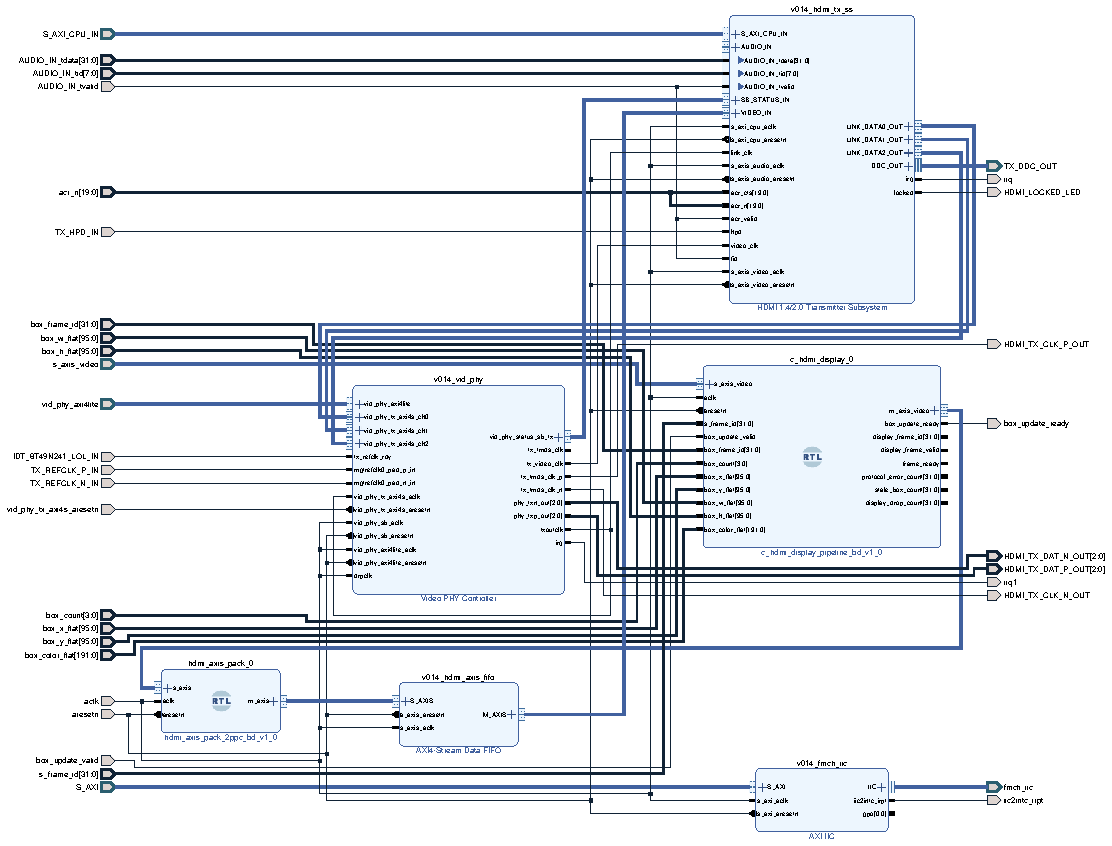
\includegraphics[width=\linewidth,height=0.66\textheight,keepaspectratio]{images/circuits/hdmi_connections.pdf}
    \caption*{图2-7（a）OSD、视频输出与 HDMI 接口实际连接（Vivado 局部视图）}
\end{figure}

\begin{figure}[H]
    \centering
    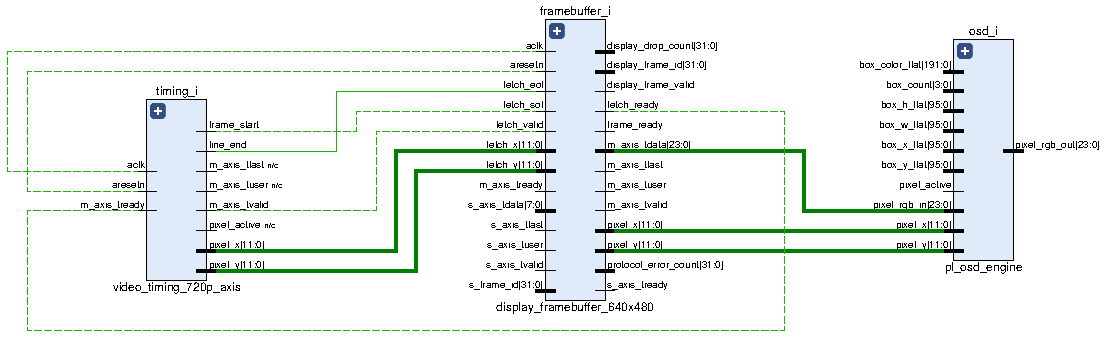
\includegraphics[width=\linewidth]{images/circuits/display_pipeline.pdf}
    \caption*{图2-7（b）视频时序、显示缓存与 OSD 的 RTL 层次连接}
\end{figure}

如图2-7所示，经过前级处理的红外图像进入显示支路。显示逻辑按照当前输出画面的像素坐标读取图像数据，并将原尺寸图像放置在指定的显示区域。随后，OSD 模块根据有效的目标框参数判断当前像素是否位于目标框边界，并在对应位置叠加颜色标记。经过 OSD 处理的图像进入 RGB888 视频数据组织模块，再由双像素打包模块将连续的两个像素组合为一个输出数据拍，最后送入 HDMI 视频输出链路。

显示过程中，系统利用 Frame ID 关联图像帧与目标框信息。当检测结果延迟返回时，不直接将旧帧检测框绘制到当前画面，而是结合当前 PL 跟踪结果维持目标位置的连续显示。这样可以避免 DPU 推理延迟造成目标框与实际目标位置不一致。

该部分的设计重点在于保证图像像素、目标框参数与显示时序之间的对应关系。PL 持续完成像素级显示处理，显示链路不必等待 DPU 每次推理完成后才输出新画面，从而保持视频输出的连续性。

\paragraph*{2. OSD 目标框叠加电路}
\subparagraph*{（1）OSD 模块组成与工作原理}
OSD（On-Screen Display）模块用于将目标框等可视化标记直接叠加到实时视频图像中。根据当前技术方案，第一版主要实现矩形目标框叠加，最多支持 8 个矩形框，边框宽度为 2 个像素，不绘制文字。

\begin{figure}[H]
    \centering
    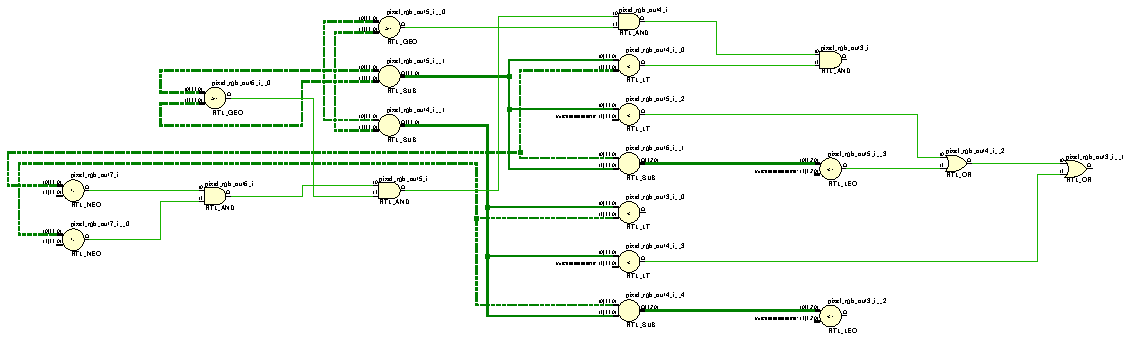
\includegraphics[width=\linewidth]{images/circuits/osd_boundary.pdf}
    \caption*{图2-8（a）OSD 坐标与边框比较电路（RTL 展开局部）}
    \vspace{8pt}
    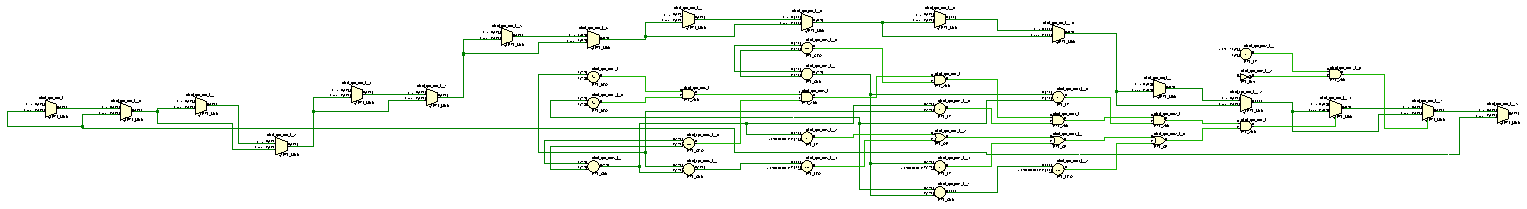
\includegraphics[width=\linewidth]{images/circuits/osd_pixel_overlay.pdf}
    \caption*{图2-8（b）OSD 边界判断与像素颜色选择电路（RTL 展开局部）}
\end{figure}

OSD 模块主要包含以下功能单元：

1. \textbf{目标框参数接收：} 接收目标框坐标、宽高、颜色、数量及对应的 Frame ID。

2. \textbf{参数缓存：} 保存当前有效的目标框参数，避免在一帧图像输出过程中参数发生变化。

3. \textbf{坐标转换：} 将原图坐标转换为输出画布坐标。

4. \textbf{矩形边界判断：} 根据当前像素坐标，判断该像素是否位于目标框边界。

5. \textbf{像素选择：} 如果当前像素位于目标框边界，则输出对应颜色；否则保留原始图像像素。

6. \textbf{视频流输出：} 将叠加后的 RGB 像素继续送入后级视频输出模块。

OSD 采用逐像素坐标比较的方式完成目标框绘制，不需要重新生成一幅完整的标注图像。对于每个有效像素，模块只需根据当前坐标和已锁存的目标框参数完成边界判断，再选择对应的输出颜色。

这种方式将目标框叠加转化为连续视频流中的局部像素替换，适合在 PL 端通过组合逻辑与流水线实现。

\subparagraph*{（2）目标框参数接口}
目标框参数来自系统当前有效的跟踪或检测状态。为保证多字段参数传输的一致性，OSD 接收接口采用有效信号与就绪信号进行握手，并在完整参数接收后更新内部参数缓存。

主要参数包括：

\begingroup\footnotesize\setlength{\tabcolsep}{4pt}\renewcommand{\arraystretch}{1.2}
\begin{longtable}{@{}>{\raggedright\arraybackslash}p{0.28\linewidth}>{\raggedright\arraybackslash}p{\dimexpr0.72\linewidth-8pt\relax}@{}}
\multicolumn{2}{c}{\textbf{目录表6 （4）视频显示输出与时序接口电路接口与信号目录}}\\\toprule
参数 & 作用\\\midrule
\endfirsthead
\multicolumn{2}{c}{\textbf{目录表6 （4）视频显示输出与时序接口电路接口与信号目录（续）}}\\\toprule
参数 & 作用\\\midrule
\endhead
\bottomrule
\endfoot
\path{box_update_valid} & 表示目标框参数有效\\\addlinespace[3pt]
\path{box_update_ready} & 表示 OSD 可以接收新参数\\\addlinespace[3pt]
\path{box_frame_id} & 标识目标框对应的图像帧\\\addlinespace[3pt]
\path{box_count} & 当前有效目标框数量，最多为 8\\\addlinespace[3pt]
\path{box_x_flat} & 各目标框左上角横坐标\\\addlinespace[3pt]
\path{box_y_flat} & 各目标框左上角纵坐标\\\addlinespace[3pt]
\path{box_w_flat} & 各目标框宽度\\\addlinespace[3pt]
\path{box_h_flat} & 各目标框高度\\\addlinespace[3pt]
\path{box_color_flat} & 各目标框的 RGB 颜色\\\addlinespace[3pt]
\end{longtable}
\endgroup

以上为接口设计字段，具体位宽、打包顺序和寄存器连接方式以最终 RTL 定义为准。

目标框参数接收完成后，OSD 将其锁存到内部参数缓存，并在显示帧边界统一更新当前使用的参数。这样可以避免在一帧图像输出过程中出现前半帧使用旧坐标、后半帧使用新坐标的情况。

\subparagraph*{（3）显示坐标转换}
当前方案采用 \(1280\times720\) 的目标显示画布，原尺寸红外图像为 \(640\times480\)。为了保持原图比例，显示时不对原图进行额外缩放，而是将图像居中放置在输出画布中。

水平方向的偏移量为：

\[
\Delta x=\frac{1280-640}{2}=320.
\]

垂直方向的偏移量为：

\[
\Delta y=\frac{720-480}{2}=120.
\]

因此，原图坐标 \((x,y)\) 转换为输出画布坐标后为：

\[
x_d=x+320,\qquad y_d=y+120.
\]

原图对应的显示区域为：

\[
320\leq x_d<960,
\]

\[
120\leq y_d<600.
\]

显示画布中其余区域输出黑色背景。

例如，原图中的目标框左上角坐标为 \((100,80)\)，转换后为：

\[
(x_d,y_d)=(420,200).
\]

由于原图没有进行缩放，目标框宽度和高度保持不变，只需对目标框位置执行相同的坐标偏移即可。

需要注意，图像坐标转换与前级检测支路的 Letterbox 坐标还原属于不同过程。检测结果在返回系统时，应先由相应的检测结果处理流程恢复到原图坐标系；OSD 再根据显示画布的布局，将原图坐标转换为最终输出坐标。

\subparagraph*{（4）矩形边界判断与像素叠加}
设目标框左上角坐标为 \((x_0,y_0)\)，宽度为 \(w\)，高度为 \(h\)。采用左闭右开的坐标约定时，目标框内部区域满足：

\[
x_0\leq x<x_0+w,
\]

\[
y_0\leq y<y_0+h.
\]

对于边框宽度为 \(t\) 的矩形框，可以通过比较当前像素与矩形四条边的距离，判断是否需要绘制边框。

以顶部边界为例，当

\[
y_0\leq y<y_0+t
\]

时，当前像素属于顶部边框区域。底部、左侧和右侧边框采用相应的坐标条件进行判断。当前方案的边框宽度设为 2 个像素。

完成边界判断后，OSD 根据判断结果选择输出像素：

- 当前像素属于有效目标框边界：输出对应目标框颜色。

- 当前像素不属于目标框边界：输出原始图像像素。

- 当前像素位于原图之外的填充区域：输出黑色背景。

对于多个目标框重叠的情况，需要在 RTL 中规定固定的处理优先级，使同一个像素在多个边框同时覆盖时仍具有确定的输出结果。

由于 OSD 只对目标框边界处的像素进行替换，其余图像内容保持不变，因此可以在保留红外图像细节的同时突出显示目标位置。

\subparagraph*{（5）目标框与显示帧的 Frame ID 校验}
目标框的位置正确，并不意味着它一定对应当前正在显示的图像。尤其是在 DPU 推理耗时较长时，检测结果可能在原始图像之后多个帧周期才返回。

为避免这种情况，系统在目标框参数中保留来源 Frame ID，并将其与当前显示帧的编号进行关联。

当检测结果返回时，系统首先确认其来源帧编号，再结合历史跟踪记录判断该结果对应的目标状态。对于当前显示帧，优先采用对应的 PL 跟踪结果进行目标框叠加；对于延迟返回的检测结果，则用于校正当前跟踪状态，而不是直接覆盖当前帧的目标坐标。

OSD 在接收新目标框参数后，还需要确认参数已经完整更新，并在合适的显示帧边界切换使用的参数。对于不符合当前显示策略的过期目标框，不直接绘制到当前画面。

通过这种方式，Frame ID 不仅用于区分不同图像，还建立了检测结果、跟踪状态和显示画面之间的时间关联，减少目标框滞后、错位和闪烁现象。

\paragraph*{3. RGB888 视频数据组织与双像素打包电路}
\subparagraph*{（1）灰度像素转换为 RGB888}
前级红外图像以 8 位灰度格式进行处理，而 HDMI 显示链路需要 RGB 格式的像素数据。因此，OSD 输出后需要将灰度像素转换为 RGB888 格式。

设输入灰度值为 \(G\)，则可以将其复制到三个颜色通道：

\[
R=G,\qquad G_{\mathrm{RGB}}=G,\qquad B=G.
\]

对应的 24 位 RGB 数据表示为：

\[
\mathrm{RGB888}
=\{R[7:0],G_{\mathrm{RGB}}[7:0],B[7:0]\}.
\]

按照当前方案的接口约定，红色、绿色和蓝色分别对应 \path{[23:16]}、\path{[15:8]} 和 \path{[7:0]}。

对于黑色背景，三个颜色通道均为 0；对于目标框边界，则直接采用 OSD 输出的颜色值。实际 RTL 需要统一 RGB 通道顺序，防止由于通道排列不一致而造成显示颜色异常。

在像素转换和 OSD 处理过程中，像素数据与 SOF、EOL、VALID 等视频流控制信号必须保持对应。若 RGB 数据经过多级流水线处理，则相关控制信号也需要经过匹配的延迟处理，以避免图像边界与像素数据错位。

\subparagraph*{（2）单像素流转换为双像素流}
根据当前方案，系统使用 \path{hdmi_axis_pack_2ppc} 模块，将 24 位单像素 RGB888 数据转换为 48 位双像素数据。

双像素模式下，每个输出数据拍包含两个连续的像素。其中，低 24 位保存第一个像素，高 24 位保存第二个像素：

\[
\mathrm{TDATA}_{48}
=\{\mathrm{Pixel}_1[23:0],\mathrm{Pixel}_0[23:0]\}.
\]

该模块需要保证两个像素的顺序正确，并使行首、行末和帧首标志与相应像素组保持一致。

对于 \(1280\times720\) 的输出画面，每行包含 1280 个像素，因此每行对应 640 个双像素数据拍。通过将两个像素组织在同一数据拍中，可以在提高每拍数据吞吐量的同时，降低内部视频处理所需的时钟频率。

双像素打包模块只负责像素数据组织和接口格式转换，不负责目标检测或目标框计算。其输出进入后级 HDMI 视频输出链路，由后续模块根据实际显示模式生成相应的输出时序。

\paragraph*{4. HDMI 视频输出与时序接口}
\subparagraph*{（1）视频输出时序}
当前方案的目标显示格式为 \(1280\times720@60\text{ Hz}\)。按照标准 720p60 视频时序，水平总周期为 1650 个像素时钟单位，垂直总周期为 750 行，对应的像素时钟为：

\[
f_{\mathrm{pixel}}
=1650\times750\times60
=74.25\ \text{MHz}.
\]

由于当前视频流采用双像素每时钟周期（2-PPC）模式，内部视频处理时钟对应为：

\[
f_{\mathrm{2PPC}}
=\frac{74.25}{2}
=37.125\ \text{MHz}.
\]

上述频率为目标显示模式下的理论时序参数，最终实际工作频率应以 HDMI 输出 IP 的配置和板端测量结果为准。

HDMI 输出链路需要正确生成有效视频区域及水平、垂直消隐等控制信息，并保证视频数据与输出时序同步。内部 AXI4-Stream 视频流中的 SOF 表示一帧有效图像的开始，EOL 表示一行有效像素的结束，两者不能直接等同于 HDMI 输出端的完整同步与消隐时序。

\subparagraph*{（2）HDMI 输出接口}
系统通过相应的视频输出 IP 和 HDMI 接口完成最终显示。显示链路需要保证 RGB 像素数据、视频有效区域、同步信息和输出时钟之间的关系正确。

HDMI 输出正常工作不仅依赖于 PL 内部生成的视频数据，还需要相应的输出时钟、接口初始化和板级连接满足要求。因此，视频时序参数、发送 IP 配置、物理接口以及相关驱动应结合实际工程进行核对。

在系统调试过程中，可以先使用固定测试图像验证 HDMI 输出时序和颜色通道，再接入真实红外视频，最后启用目标框叠加功能。通过逐步增加模块，可以区分图像数据错误、OSD 坐标错误和 HDMI 时序配置错误，便于定位问题。

\paragraph*{5. 时钟、跨时钟域与复位接口}
\subparagraph*{（1）时钟域划分}
系统视频链路可能涉及摄像头像素时钟、PL 内部视频处理时钟、AXI 总线时钟以及 HDMI 输出时钟。不同模块的时钟频率和相位可能不同，因此需要依据实际工程明确各模块的时钟归属。

对于同一时钟域内的像素处理模块，可以通过同步流水线传递数据与控制信号。对于跨时钟域的视频流，则需要采用经过验证的异步 FIFO 或相应的官方跨时钟域结构，不能直接对多位像素总线进行异步采样。

跨时钟域处理时，像素数据与 SOF、EOL 等边界信息应作为一个整体进行传递，确保读出端能够正确恢复原有视频流结构。

\subparagraph*{（2）跨时钟域控制信息}
目标框坐标、Frame ID 和跟踪状态等信息可能与显示像素处于不同的时钟域。对于这些多位数据，需要通过握手、稳定数据保持或其他经过验证的跨时钟域机制完成传输，避免不同字段在不同时间被采样。

单比特状态信号可以采用适当的同步器；多位参数则不能简单地对每一位分别使用同步触发器后直接组合，因为这样可能导致接收到的参数并非同一组完整数据。

目标框参数应在完整接收后统一锁存，并在适当的帧边界更新。这样可以使 OSD 在一帧图像的输出过程中始终使用一致的坐标和颜色参数。

\subparagraph*{（3）复位与初始化}
显示链路的复位需要覆盖 OSD 控制逻辑、视频格式转换、双像素打包及相关跨时钟域接口。复位释放后，各模块应恢复到确定的初始状态，并等待有效视频帧和有效目标框参数。

OSD 在初始化阶段应将目标框数量置为 0，避免将未初始化的坐标数据作为有效目标框绘制；视频打包模块应重新建立像素组边界，避免复位前残留的数据影响后续输出。

对于跨时钟域模块，应根据各时钟域的实际情况完成复位同步释放。HDMI 输出链路则需要按照所使用 IP 的要求完成时钟建立和接口初始化，再进入正常视频输出状态。

\paragraph*{6. 关键输入输出信号与接口关系}
显示输出与时序接口的主要信号关系如下。

\begingroup\footnotesize\setlength{\tabcolsep}{4pt}\renewcommand{\arraystretch}{1.2}
\begin{longtable}{@{}>{\raggedright\arraybackslash}p{0.18\linewidth}>{\raggedright\arraybackslash}p{0.25\linewidth}>{\raggedright\arraybackslash}p{0.25\linewidth}>{\raggedright\arraybackslash}p{\dimexpr0.32\linewidth-24pt\relax}@{}}
\multicolumn{4}{c}{\textbf{目录表7 （4）视频显示输出与时序接口电路接口与信号目录}}\\\toprule
模块 & 关键输入 & 关键输出 & 主要作用\\\midrule
\endfirsthead
\multicolumn{4}{c}{\textbf{目录表7 （4）视频显示输出与时序接口电路接口与信号目录（续）}}\\\toprule
模块 & 关键输入 & 关键输出 & 主要作用\\\midrule
\endhead
\bottomrule
\endfoot
OSD 参数接收 & 目标框坐标、宽高、颜色、Frame ID & 锁存后的目标框参数 & 接收并保存有效显示参数\\\addlinespace[3pt]
坐标转换 & 原图坐标、画布偏移量 & 显示画布坐标 & 将原图位置映射到输出画布\\\addlinespace[3pt]
矩形边界判断 & 当前像素坐标、目标框参数 & 边界命中标志 & 判断当前像素是否需要叠加\\\addlinespace[3pt]
像素选择 & 原始灰度像素、目标框颜色、边界命中标志 & 叠加后的像素 & 完成目标框绘制\\\addlinespace[3pt]
Frame ID 校验 & 当前显示帧编号、目标框来源帧编号 & 参数有效状态 & 避免直接使用不适用的旧目标框\\\addlinespace[3pt]
RGB888 转换 & 8 位灰度像素或 OSD 颜色 & 24 位 RGB 数据 & 组织三通道显示数据\\\addlinespace[3pt]
双像素打包 & 24 位单像素 RGB 数据 & 48 位双像素数据 & 完成 2-PPC 数据组织\\\addlinespace[3pt]
HDMI 视频输出 & RGB 视频流、有效信号、同步控制及时钟 & HDMI 视频输出 & 完成最终显示接口输出\\\addlinespace[3pt]
\end{longtable}
\endgroup

综上，视频显示输出与时序接口电路通过 PL 端 OSD 目标框叠加、坐标转换、RGB888 数据组织和双像素打包，完成从处理后红外图像到 HDMI 视频输出的转换。系统结合 Frame ID 校验与帧边界参数更新机制，保证目标框和显示图像之间的对应关系，并通过合理的时钟、跨时钟域与复位设计，保障视频数据在输出链路中的正确传输，为实时目标检测与连续跟踪结果的可视化提供支持。

\subsubsection*{电路接口与信号表格目录}
\begingroup\footnotesize\setlength{\tabcolsep}{4pt}\renewcommand{\arraystretch}{1.2}
\begin{longtable}{@{}>{\raggedright\arraybackslash}p{0.18\linewidth}>{\raggedright\arraybackslash}p{0.25\linewidth}>{\raggedright\arraybackslash}p{0.25\linewidth}>{\raggedright\arraybackslash}p{\dimexpr0.32\linewidth-24pt\relax}@{}}
\multicolumn{4}{c}{\textbf{目录表4 （3）DPU 检测数据通路与 PS—PL 控制接口电路接口与信号目录}}\\\toprule
偏移地址 & 寄存器名称 & 方向 & 功能说明\\\midrule
\endfirsthead
\multicolumn{4}{c}{\textbf{目录表4 （3）DPU 检测数据通路与 PS—PL 控制接口电路接口与信号目录（续）}}\\\toprule
偏移地址 & 寄存器名称 & 方向 & 功能说明\\\midrule
\endhead
\bottomrule
\endfoot
\path{0x00} & \path{CTRL} & PS→PL & 系统使能、软复位和工作模式\\\addlinespace[3pt]
\path{0x04} & \path{STATUS} & PL→PS & 当前状态、错误标志及缓冲区状态\\\addlinespace[3pt]
\path{0x08} & \path{FRAME_ID} & PL→PS & 最新完整帧编号\\\addlinespace[3pt]
\path{0x0C} & \path{REQUEST_SEQ} & PL→PS & 检测请求序号\\\addlinespace[3pt]
\path{0x10} & \path{DETECT_FRAME_ID} & PS→PL & 检测结果对应的来源帧编号\\\addlinespace[3pt]
\path{0x14} & \path{DETECT_XY} & PS→PL & 检测框左上角坐标\\\addlinespace[3pt]
\path{0x18} & \path{DETECT_WH} & PS→PL & 检测框宽度和高度\\\addlinespace[3pt]
\path{0x1C} & \path{DETECT_CONF} & PS→PL & 检测置信度\\\addlinespace[3pt]
\path{0x20} & \path{RESULT_SEQ} & PS→PL & 检测结果提交序号\\\addlinespace[3pt]
\path{0x24} & \path{TRACK_XY} & PL→PS & 当前跟踪框坐标\\\addlinespace[3pt]
\path{0x28} & \path{TRACK_SCORE} & PL→PS & SAD 匹配误差和唯一性指标\\\addlinespace[3pt]
\path{0x2C} & \path{TRACK_STATE} & PL→PS & 当前跟踪状态\\\addlinespace[3pt]
\path{0x30} & \path{REDTECT_PERIOD} & PS→PL & 周期重检测间隔\\\addlinespace[3pt]
\path{0x34} & \path{FRAME_AGE} & PL→PS & 当前检测结果帧龄\\\addlinespace[3pt]
\path{0x38} & \path{DROP_COUNT} & PL→PS & 过期帧和异常帧计数\\\addlinespace[3pt]
\path{0x3C} & \path{ERROR_CODE} & PL→PS & 错行、溢出和超时等错误状态\\\addlinespace[3pt]
\path{0x40} & \path{BUFFER_ID} & 双向 & 请求与结果关联的缓冲区编号\\\addlinespace[3pt]
\path{0x44} & \path{REQUEST_REASON} & PL→PS & 周期检测、低可信度或目标丢失等请求原因\\\addlinespace[3pt]
\end{longtable}
\endgroup

\Needspace{3\baselineskip}
\section*{2.3 软件系统介绍}

\Needspace{3\baselineskip}
\subsection*{2.3.1 软件整体介绍}

软件由PC离线开发部署环境、PS运行控制与模型服务、硬件结果适配及监测三部分组成。PC完成模型训练、量化、编译和硬件工程构建，运行时摄像头向PL连续供给视频；PS只配置摄像头和硬件、处理检测请求及管理结果。逐像素增强、SAD和OSD由PL执行，软件流程不重复实现硬件流水线。

% PPT P7
\begin{figure}[H]
    \centering
    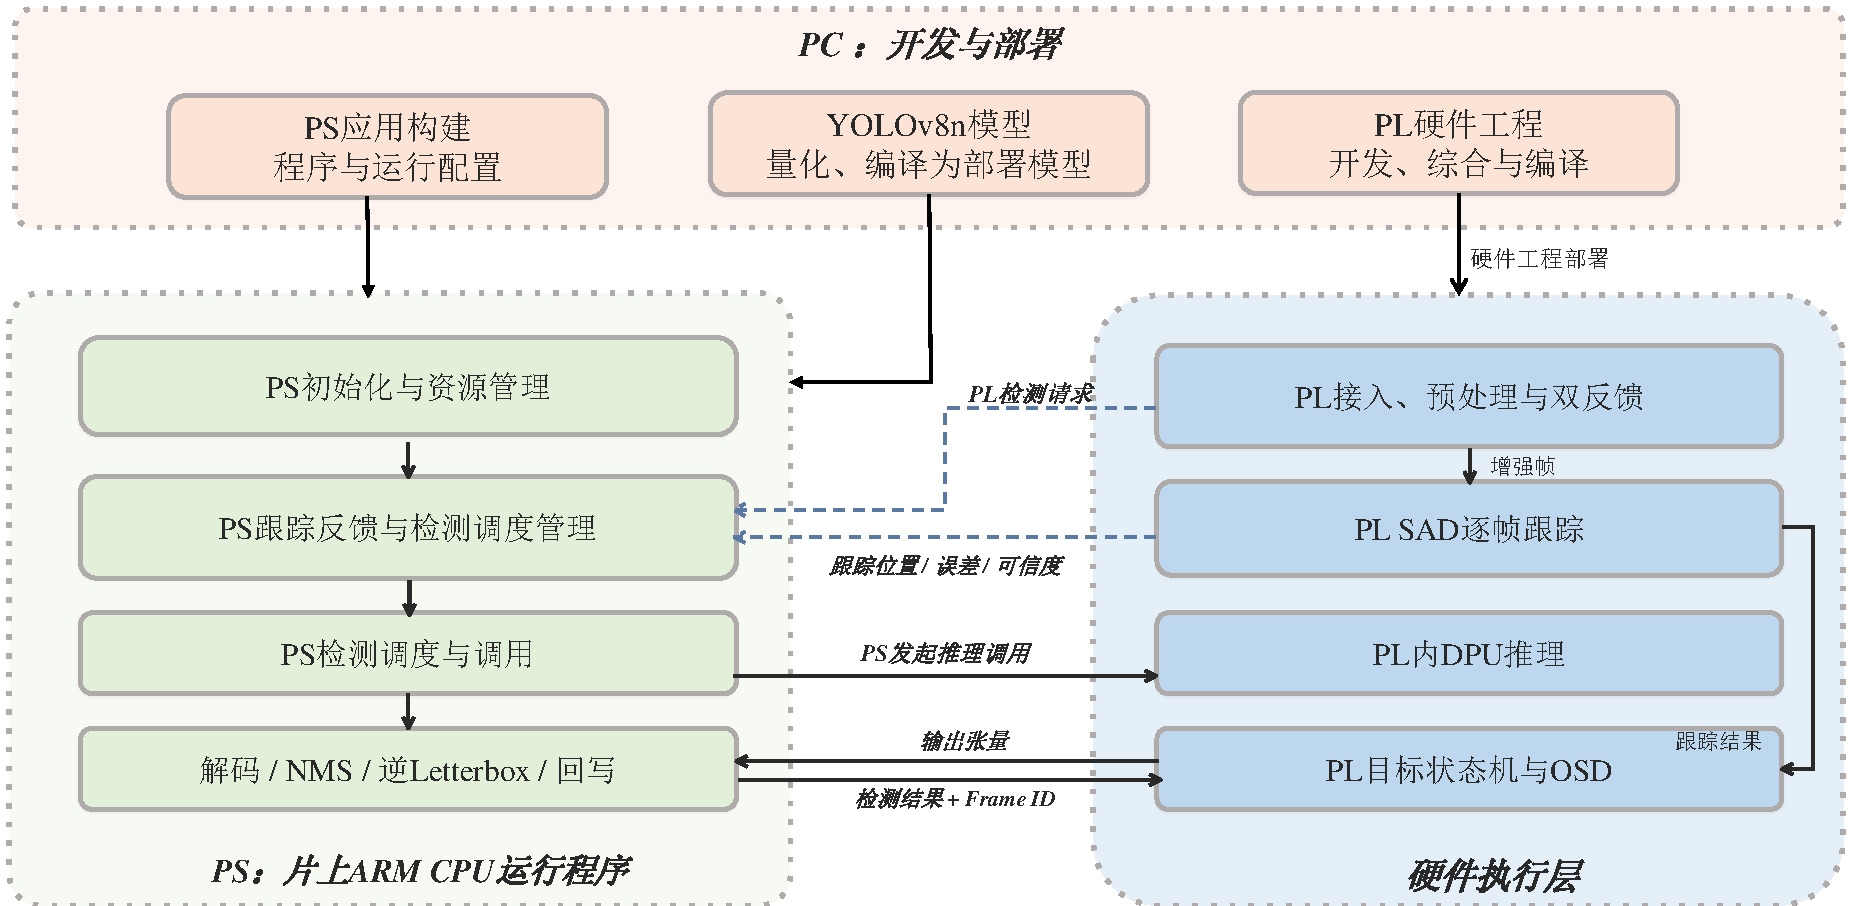
\includegraphics[
        width=\linewidth,
        height=0.60\textheight,
        keepaspectratio
    ]{images/flowcharts/p07.pdf}
    \caption{软件系统总体架构图}
    \label{fig:software}
\end{figure}

软件架构图上层为离线工具与部署文件，中层为PS初始化、请求服务、推理和后处理，下层为PL执行模块。PS与PL之间主要传递控制、帧身份和结果信息，图像主体由摄像头和硬件帧链产生。模型文件、bit/hwh/xclbin及应用程序已按同一目标平台版本管理，并完成与合并系统镜像的匹配检查。

PC参考预处理以640×640×3、RGB、保持比例、最近邻插值和补边114为约定，可用于对照PL输出。部署时依实际Tensor布局和量化参数准备模型输入，不能把DDR四字节R/G/B/0直接视为RGB三通道Tensor。NMS按类别处理，\path{inverse_letterbox}()恢复原图坐标；固定输入情形缩放比例为1，Y坐标去除80行补边后裁剪。


\Needspace{3\baselineskip}
\subsection*{2.3.2 软件各模块介绍}

% PPT P8
\begin{figure}[H]
    \centering
    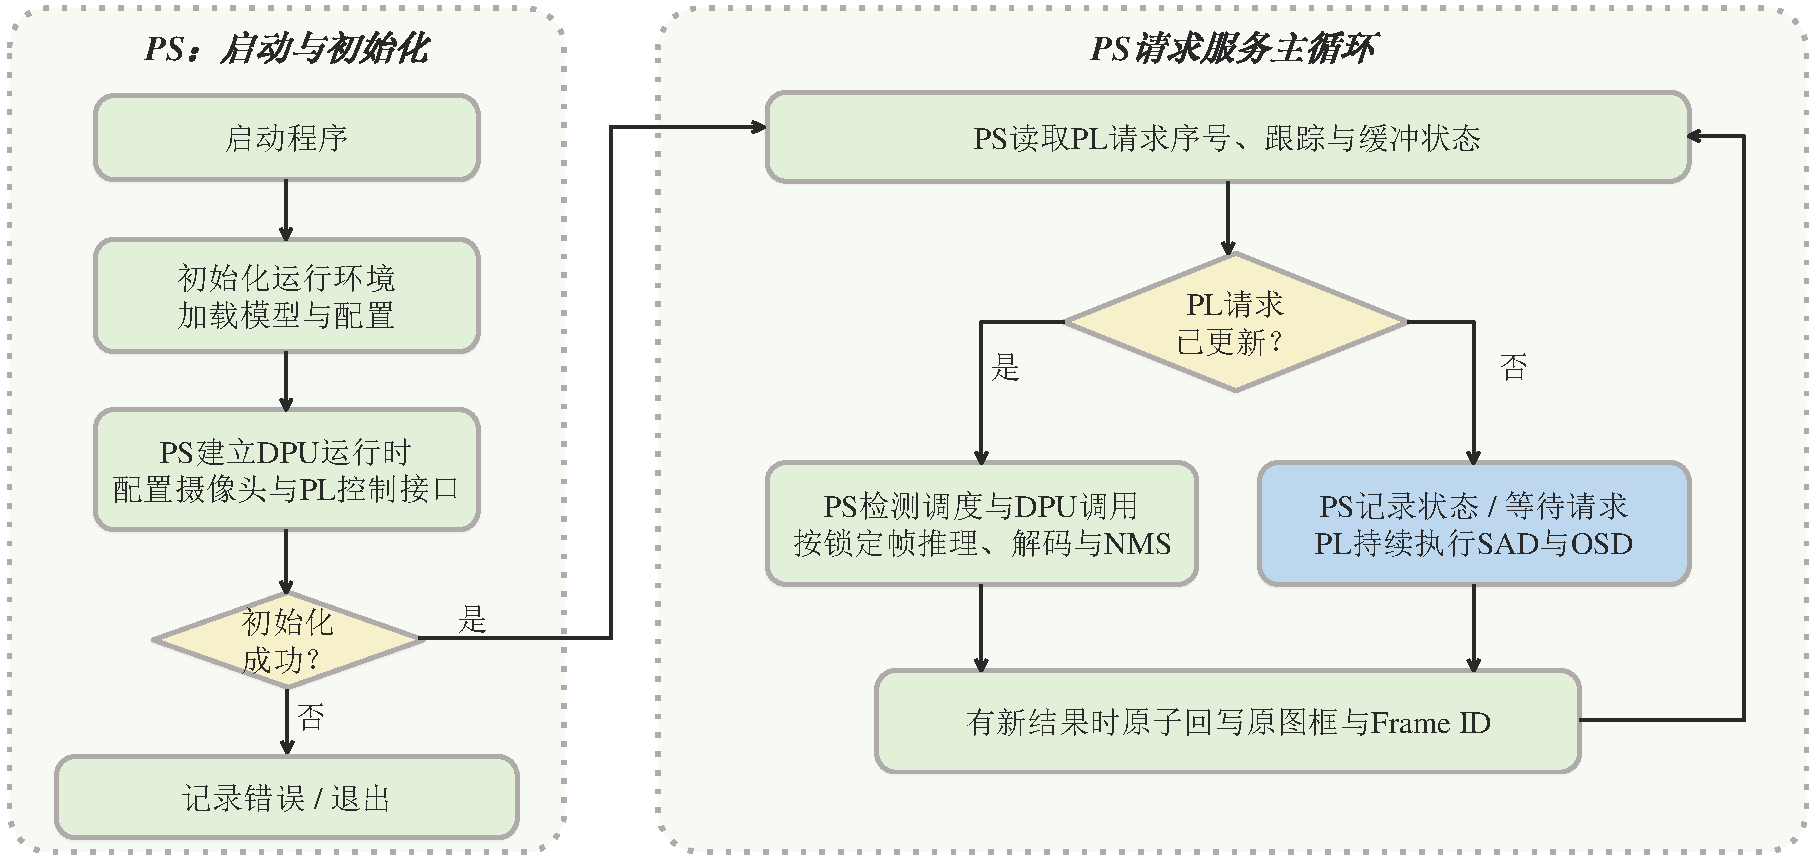
\includegraphics[
        width=\linewidth,
        height=0.60\textheight,
        keepaspectratio
    ]{images/flowcharts/p08.pdf}
    \caption{PS 端程序主流程图}
    \label{fig:ps-main}
\end{figure}
\Needspace{3\baselineskip}

\subsubsection*{（1）初始化、主循环与资源管理}

启动时先关闭流水线，检查硬件版本和模型文件，确认DDR保留区、地址映射及缓存一致性策略，初始化摄像头控制接口、DPU运行时、邮箱和统计模块；摄像头输出稳定且PL采样和同步配置有效后再使能处理链。初始化失败应输出可定位的错误并退出，避免在未保留内存或错误时钟条件下写帧。



主流程图将一次性初始化与循环服务分开：进入主循环后，PS读取请求序号、跟踪反馈及缓冲状态；有新请求才调度DPU，无新请求则记录状态或等待事件。PL持续处理摄像头图像，不等待一次推理完成。推理结果以来源Frame ID及缓冲身份回写，因此软件响应时刻不能代替图像采集时刻。

关键输入包括摄像头参数、模型与Overlay路径、控制基址、阈值及超时配置；关键输出包括初始化状态、运行时对象、统计快照和错误码。停止时先阻止新请求与新帧事务，再按受控顺序排空或恢复，最后释放软件资源。运行日志应记录硬件版本、模型校验值、来源帧号、请求序号及异常原因。


\Needspace{3\baselineskip}
\subsubsection*{（2）请求读取与检测调度}
% PPT P9
\begin{figure}[H]
    \centering
    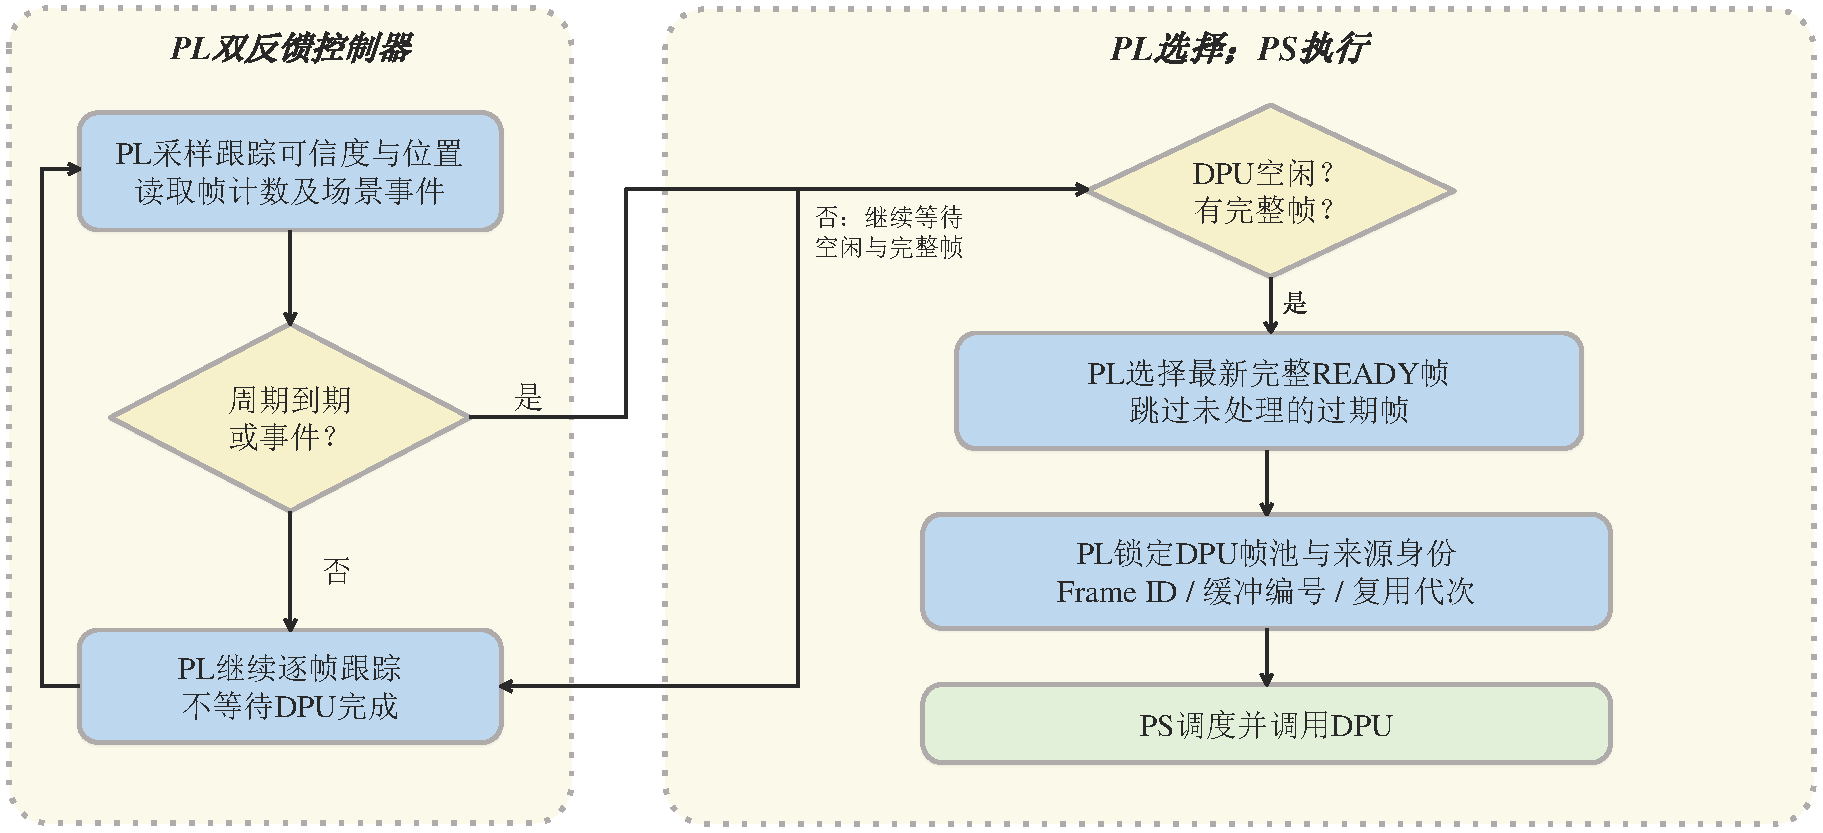
\includegraphics[
        width=\linewidth,
        height=0.60\textheight,
        keepaspectratio
    ]{images/flowcharts/p09.pdf}
    \caption{检测任务调度流程图}
    \label{fig:dispatch}
\end{figure}
调度依据周期、跟踪可信度、目标丢失和场景变化等事件生成检测需求。需求并不直接意味着可调用DPU，必须同时满足推理可接受和存在完整READY帧。PL锁定最新帧及其\path{buffer_id}和generation后发布请求，PS通过序号前后复读获得一致快照并确认中断。推理进行中保留连续跟踪，随后以新鲜完整帧服务下一次请求。



调度图左侧描述PL产生需求，右侧描述等待可用帧、最新帧选择和PS执行。将“需要检测”与“能够发起检测”分开，可避免重复调用、读取半帧或覆写DPU所有权。未满足条件时继续接收和跟踪；符合条件时一次性发布来源帧身份。事件优先级、节流与原因编码已在集成版本中统一，调度顺序由状态条件确定。

关键输入为\path{REQUEST_SEQ}、请求三元组、reason、timestamp及\path{IRQ_STATUS}，输出为一致请求快照和选定推理帧。异常请求、重复序号与超时应有独立日志。超时恢复先确认硬件消费者状态，再按所有权协议回收，不能在DPU仍可能访问图像时直接复用缓冲。


\Needspace{3\baselineskip}
\subsubsection*{（3）DPU调用、后处理与原子提交}
% PPT P10
\begin{figure}[H]
    \centering
    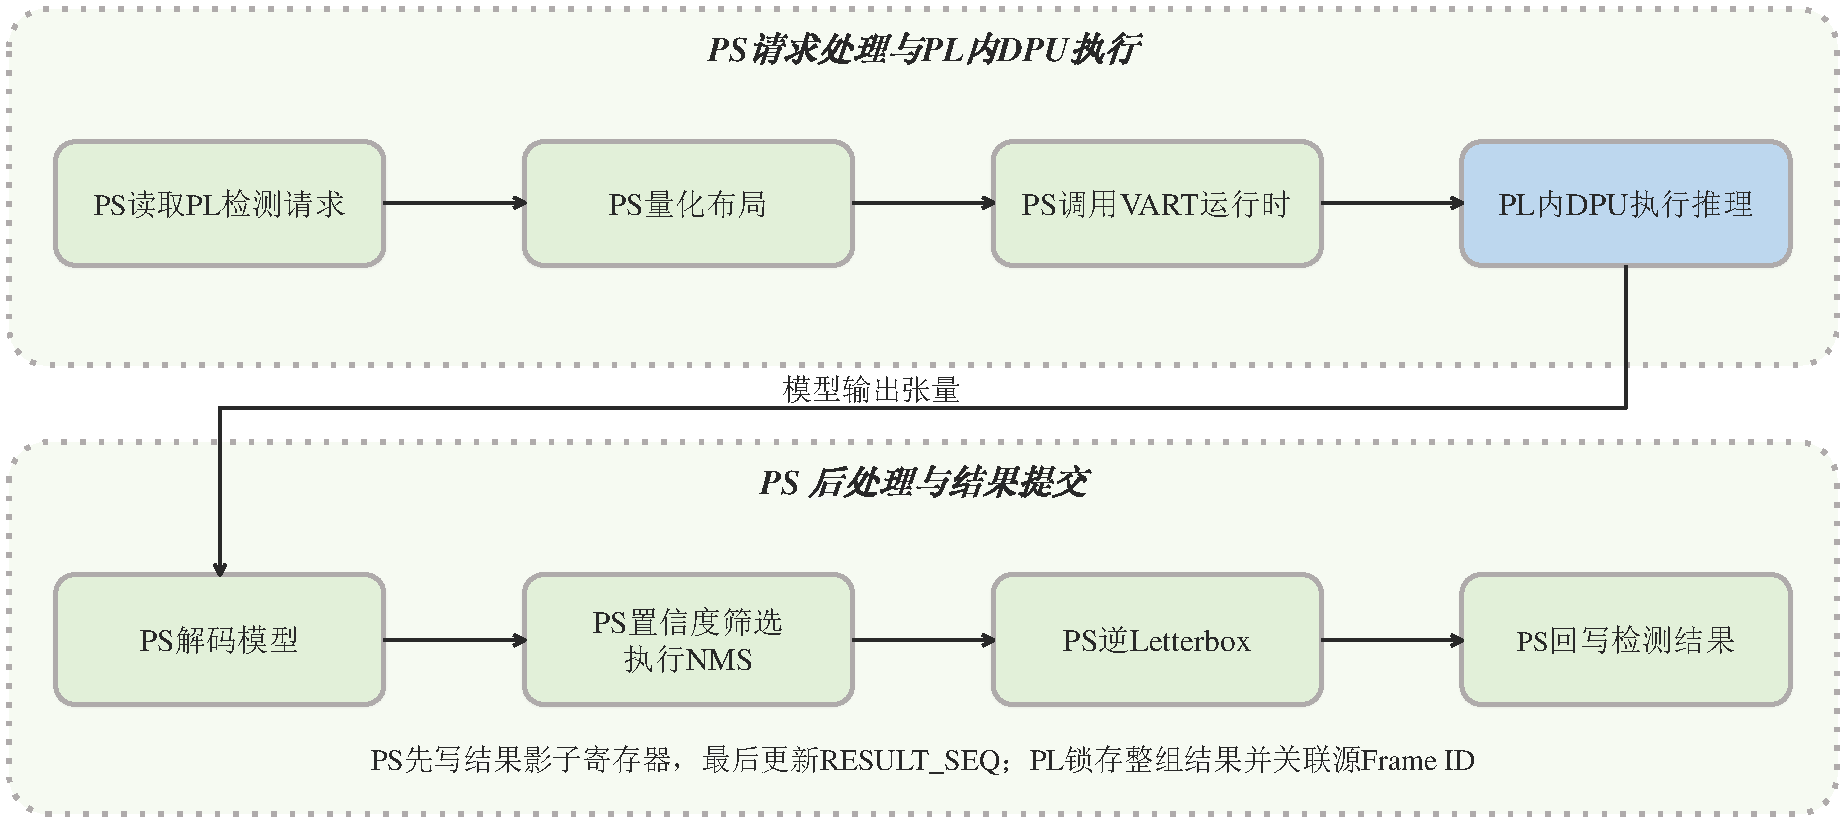
\includegraphics[
        width=\linewidth,
        height=0.60\textheight,
        keepaspectratio
    ]{images/flowcharts/p10.pdf}
    \caption{DPU 推理调用与后处理流程图}
    \label{fig:inference}
\end{figure}
PS先检查部署包与实际DPU架构匹配，再从锁定帧准备Tensor，调用VART运行时并读取输出。已有部署资料包含dpu.zcu104.2.5.0.bit及其hwh、xclbin，模型\path{tank_yolov8n_relu_finetuned_100_fixed.xmodel}的记录MD5为3eaee0e293cef1a2cc69b811b5c5f0fe；\path{board_runner_probe.py}提供Overlay、模型、Tensor元数据和量化参数检查。部署检查完成后，已进一步完成板端推理、后处理及摄像头输入到显示输出的整机验证。

后处理按模型实际输出完成框解码、置信度筛选、按类别NMS、坐标逆变换及边界裁剪。无目标、超时和错误应使用对应结果状态。结果继承原请求的来源帧号、缓冲编号和代次，置信度按接口转换为Q0.16；影子字段全部写完后才发出原子提交。



图中上排为PS请求准备和DPU执行，下排为模型输出解码、NMS、逆Letterbox及回写。该图放在推理与后处理的联合模块中，以便按实际调用顺序说明数据转换。原图“最后更新\path{RESULT_SEQ}”应按接口协议理解为结果发布后的序号变化：PS最后写的是\path{RESULT_COMMIT}=1，\path{RESULT_SEQ}由PL硬件递增，软件不得直接写该寄存器。

关键输入是请求帧身份、模型输入Tensor、输出Tensor及置信度与IoU阈值；输出是原图坐标框、类别、置信度和结果状态。完成三元组匹配才结束活动请求并释放帧池；不匹配时记录过期结果。对应来源帧的检测用于状态校正，当前帧位置必须由已有历史或跟踪信息推导。


\Needspace{3\baselineskip}
\subsubsection*{（4）显示适配、监测与异常处理}

软件或PL适配层把结果打包为最多8个显示slot，提交帧号、X/Y/W/H及RGB颜色，整包保持到valid/ready握手完成。显示侧框bank与图像bank按帧边界切换，未匹配的旧框不显示。多框提交的控制通路、PS适配和显示封装已完成联调，框配置按完整数据包握手发布。

监测模块捕获统一统计快照，分别记录视频帧完成、写事务成功或失败、检测请求、合法结果释放、显示丢帧和旧框拒绝。请求到\path{result_release}的周期差包含PS准备、推理、后处理和提交，是请求往返延迟；纯推理时间需在运行时单独计时。摄像头丢同步、写事务失败、推理超时和显示协议错误应分别记录，并通过受控复位或重同步恢复。

运行程序按资源初始化、请求服务、模型执行、后处理、结果提交和显示适配分层组织。各层通过运行时对象、请求快照、Tensor及结果结构传递数据，已完成正常路径和异常路径联调；PL算法计算由硬件持续执行，不作为PS逐帧函数调用。


\Needspace{3\baselineskip}
\section*{第三部分 完成情况及性能参数}

\subsection*{3.1 整体介绍}

系统已按既定计划完成硬件设计、软件开发、模块验证、统一主工程集成和实板联调，形成红外摄像头输入、PL校正增强、SAD逐帧跟踪、DPU按需检测、结果校正与HDMI标注显示的完整闭环。摄像头像素直接进入PL，连续视频处理与间歇检测并行运行，PS负责配置、推理调用和后处理。

整机由红外摄像头、ZCU104、供电散热和显示终端组成，已完成接口连接、设备固定与运行配置。系统运行时能够连续输出带目标框的视频画面，检测、跟踪、帧池和显示状态通过统一日志及监测接口关联，满足从模块调试到整机运行的检查需求。


\subsection*{3.2 工程成果}

\subsubsection*{3.2.1 机械与安装成果}

已完成摄像头、开发板、显示终端及线缆的安装和连接，保证摄像头视轴稳定、连接器固定、供电匹配与板卡散热。设备布局便于观察显示结果和连接调试接口，连续运行中保持采集与显示链路稳定。作品采用标准开发板，机械成果为实际原型安装与系统布置。


\subsubsection*{3.2.2 电路与硬件成果}

已完成摄像头采样、帧同步、跨域传输、校正增强、SAD、双反馈控制、Letterbox、DataMover写帧、三缓冲及显示链的集成。各模块使用统一帧身份，并按所有权和原子提交协议交互。合并工程已完成综合、实现、DRC、CDC和时序检查，并导出相互匹配的硬件交付文件。

\begingroup
\footnotesize
\setlength{\tabcolsep}{4pt}
\renewcommand{\arraystretch}{1.2}

\begin{longtable}{@{}
    >{\raggedright\arraybackslash}p{0.21\linewidth}
    >{\raggedright\arraybackslash}p{0.39\linewidth}
    >{\raggedright\arraybackslash}p{\dimexpr0.40\linewidth-16pt\relax}
@{}}
\multicolumn{3}{c}{
    \normalsize\textbf{表3-1 工程完成情况}
}\\[6pt]
\toprule
项目 & 完成内容 & 实现结果 \\
\midrule
\endfirsthead

\multicolumn{3}{c}{
    \normalsize\textbf{表3-1 工程完成情况（续）}
}\\[6pt]
\toprule
项目 & 完成内容 & 实现结果 \\
\midrule
\endhead

\bottomrule
\endfoot

采集与同步
& 摄像头接入、像素格式适配、帧边界和跨域处理
& 连续采集并向PL处理链提供完整有效帧。 \\
\addlinespace[3pt]

校正与增强
& 非均匀性校正、场景统计与空间自适应增强
& 完成流式处理和帧边界参数更新。 \\
\addlinespace[3pt]

检测与跟踪
& SAD逐帧跟踪、DPU检测、NMS及状态校正
& 完成目标初始化、连续定位和异常重检闭环。 \\
\addlinespace[3pt]

三缓冲与帧调度
& Fresh-Frame选择、三元组身份校验与原子提交
& 完成最新完整帧服务、所有权保护和旧结果拒绝。 \\
\addlinespace[3pt]

显示与OSD
& 独立双帧缓存、框身份匹配、2-PPC及HDMI链
& 完成720p视频标注输出与缓存边界切换。 \\
\addlinespace[3pt]

主工程与软件
& 统一BD、时序及跨域检查、驱动与应用
& 完成软硬件同版交付和实板联调。 \\
\addlinespace[3pt]

运行与恢复
& 监测快照、日志、超时和错误恢复
& 完成连续运行及异常处理验证。 \\
\addlinespace[3pt]

\end{longtable}
\endgroup


\subsubsection*{3.2.3 软件与部署成果}

已完成模型训练、硬件适配、INT8量化、模型编译及板端部署，运行时核对Tensor布局、量化参数和硬件平台。PS程序完成初始化、摄像头配置、请求服务、推理、解码、NMS、逆Letterbox和原子结果提交，显示适配和监测程序能够关联图像与目标状态。

软件与硬件文件已按版本统一整理，运行日志覆盖来源帧号、请求序号、缓冲编号、复用代次、推理结果和错误状态。系统完成正常运行、重复请求、过期结果、资源忙、推理超时和受控恢复等路径的联调，构成可运行的完整工程成果。


\subsection*{3.3 功能与性能验证结果}

系统验证已围绕采集、增强、检测跟踪、缓存调度、显示输出和异常恢复完成。表3-2按测试内容和功能结果归纳，性能配置见表1-1。帧率、精度、延迟及功耗采用原始测试记录的统计口径，本文不新增未经提供的测量数字。

\begingroup
\footnotesize
\setlength{\tabcolsep}{4pt}
\renewcommand{\arraystretch}{1.2}

\begin{longtable}{@{}
    >{\raggedright\arraybackslash}p{0.21\linewidth}
    >{\raggedright\arraybackslash}p{0.39\linewidth}
    >{\raggedright\arraybackslash}p{\dimexpr0.40\linewidth-16pt\relax}
@{}}
\multicolumn{3}{c}{
    \normalsize\textbf{表3-2 系统功能与性能验证结果}
}\\[6pt]
\toprule
验证项目 & 检查内容 & 完成结果 \\
\midrule
\endfirsthead

\multicolumn{3}{c}{
    \normalsize\textbf{表3-2 系统功能与性能验证结果（续）}
}\\[6pt]
\toprule
验证项目 & 检查内容 & 完成结果 \\
\midrule
\endhead

\bottomrule
\endfoot

摄像头输入
& 连续像素、SOF/EOL、帧计数及跨域数据
& 完成连续采集、帧同步及异常帧恢复验证。 \\
\addlinespace[3pt]

图像预处理
& 校正、动态范围拉伸、细节增强及参数锁存
& 完成流水处理和增强前后图像对照检查。 \\
\addlinespace[3pt]

检测后处理
& 模型调用、Tensor布局、解码、NMS与坐标还原
& 完成板端检测及原图坐标结果输出。 \\
\addlinespace[3pt]

连续跟踪
& 目标初始化、SAD位置更新、模板切换和重检
& 完成检测间隔内逐帧定位及状态恢复。 \\
\addlinespace[3pt]

帧调度
& READY选择、DPU\_OWNED保护、generation及返回身份
& 完成最新完整帧选择和资源所有权检查。 \\
\addlinespace[3pt]

显示一致性
& 双bank发布、框Frame ID、OSD及HDMI输出
& 完成图像帧边界切换和目标标注显示。 \\
\addlinespace[3pt]

工程与运行
& 实现、时序、跨域、驱动和整机连续运行
& 完成统一工程与板端闭环验证。 \\
\addlinespace[3pt]

异常恢复
& 丢同步、写失败、超时、旧结果和输出状态
& 完成异常记录、重同步及受控恢复验证。 \\
\addlinespace[3pt]

\end{longtable}
\endgroup

验证中分别统计输入帧、成功写入帧、检测结果和显示帧，避免把累计帧计数直接视为FPS，也不以显示刷新率替代检测速度。请求到合法结果释放的时间包含准备、推理、后处理和提交，摄像头到显示的延迟还包含缓存发布等待。结果帧龄与显示帧龄均在统一来源Frame ID域中计算，保证性能结论对应同一数据路径。

通过上述工作，系统已完成由单模块到整机的验证闭环。最终交付包含同版硬件文件、模型和应用、接口说明及运行记录，能够对应说明摄像头输入、检测跟踪协同和标注显示的实际运行过程。


\section*{第四部分 总结}

\Needspace{3\baselineskip}
\section*{4.1 可扩展之处}

\begin{enumerate}
    \item \textbf{输入适配扩展：}
    扩展摄像头适配及多分辨率输入，建立不同采样时钟和像素格式下的稳定接入机制。

\item \textbf{检测跟踪扩展：}
    增加多目标身份管理、遮挡恢复和运动预测，提高复杂场景下连续定位的稳定性。

    \item \textbf{复杂场景优化：}
    针对低对比度、背景变化和热交叉场景优化增强与跟踪参数，并联合训练及量化校准评估检测效果。

    

    \item \textbf{自适应检测调度：}
    依据跟踪可信度、场景变化及系统负载动态调整检测周期，协调定位效果与推理开销。

    \item \textbf{系统性能优化：}
    在现有统一Frame ID、历史校正、驱动和恢复机制基础上，进一步优化资源、功耗及端到端延迟，面向更复杂场景扩展系统能力。
\end{enumerate}


\Needspace{3\baselineskip}
\section*{4.2 心得体会}

本项目使我们认识到，红外视觉系统的设计需要把图像质量、定位效果和数据时效性放在同一条处理链上考虑。摄像头直接接入PL后，输入像素并不等待软件任务完成，采样、跨域、缓存和错误帧恢复与算法本身同样重要。只有先把帧首、行末、像素格式和有效条件定义清楚，后续预处理、跟踪和检测才有可信的数据基础。

在预处理设计中，灰度拉伸和细节增强不能只依据显示效果评价。增强过强会放大噪声，也可能改变模型习惯的数据分布，因此需要在图像可辨识性、检测表现、定点精度和硬件成本之间反复比较。将第N帧统计用于第N+1帧，并在帧首锁存参数，使我们更加重视动态控制与流水线一致性的关系。

检测与跟踪的分工让我们从系统效率而非单一推理速度出发思考实时性。PL通过SAD维持相邻帧位置，DPU按需提供检测校准，能够减少持续定位对每帧深度推理的依赖；但异步检测带来历史结果如何校正当前状态的问题。帧号、缓存代次、所有权和原子提交并非附加标签，而是防止系统在运行中使用错误图像和旧结果的基本条件。

设计流程图和接口表的整理也暴露了工程文档之间容易出现的差异：像素流与整帧写事务结束、目标显示制式与检测FPS、模块仿真通过与实板闭环完成，分别属于不同层面的结论。我们需要将设计目标、实现接口和验证证据逐项对应，避免用一张完整框图代替实际成果。通过完成统一主工程、摄像头采样、跨域、板端推理和连续输出联调，我们将算法设计、硬件实现和验证记录对应起来，形成可运行、可检查的工程结果，也加深了对软硬件协同开发的理解。


\Needspace{3\baselineskip}
\section*{第五部分 参考文献}

\begingroup
\footnotesize
\setlength{\parskip}{2pt}

[1] AMD. ZCU104 Evaluation Board User Guide (UG1267)[EB/OL]. 2018-10-09[2026-10-21]. \url{https://docs.amd.com/v/u/en-US/ug1267-zcu104-eval-bd}.

[2] AMD. AXI4-Stream Video IP and System Design Guide (UG934)[EB/OL]. 2022-11-16[2026-10-21]. \url{https://docs.amd.com/r/en-US/ug934_axi_videoIP}.

[3] AMD. Vitis AI User Guide (UG1414), Version 2.5[EB/OL]. 2022-06-15[2026-10-21]. \url{https://docs.amd.com/r/2.5-English/ug1414-vitis-ai}.

[4] AMD. DPUCZDX8G for Zynq UltraScale+ MPSoCs Product Guide (PG338)[EB/OL]. \url{https://docs.amd.com/r/en-US/pg338-dpu}.

[5] WANG X, HE X, ZHU X, et al. Lightweight and Real-Time Infrared Image Processor Based on FPGA[J]. Sensors, 2024, 24(4): 1333. DOI: 10.3390/s24041333.

[6] LI T, CHEN X. FPGA Implementation of Real-Time Processing of Infrared Focal Plane Images[J]. Infrared, 2023, 44(7): 15-20.

[7] LEE T J, LIU Y W, LIN Y C. Real-time IR Image Processing Interface on FPGA with Histogram Equalization and Non-Uniform Correction[C]//2023 International Conference on Consumer Electronics-Taiwan (ICCE-Taiwan). IEEE, 2023: 709-710. DOI: 10.1109/ICCE-Taiwan58799.2023.10226928.

[8] SINGH S, SHEKHAR C, VOHRA A. Real-Time FPGA-Based Object Tracker with Automatic Pan-Tilt Features for Smart Video Surveillance Systems[J]. Journal of Imaging, 2017, 3(2): 18. DOI: 10.3390/jimaging3020018.

[9] HU T, WU H, IKENAGA T. FPGA Implementation of High Frame Rate and Ultra-Low Delay Tracking with Local-Search Based Block Matching[C]//2017 International Conference on Machine Vision and Information Technology (CMVIT). IEEE, 2017: 93-98. DOI: 10.1109/CMVIT.2017.24.

[10] WILLIAMS J, MIKHELSON I. Triple Frame Buffer FPGA Implementation[J]. HardwareX, 2019, 5: e00064. DOI: 10.1016/j.ohx.2019.e00064.

\endgroup

\clearpage
\begin{landscape}
\begin{figure}[p]
    \centering
    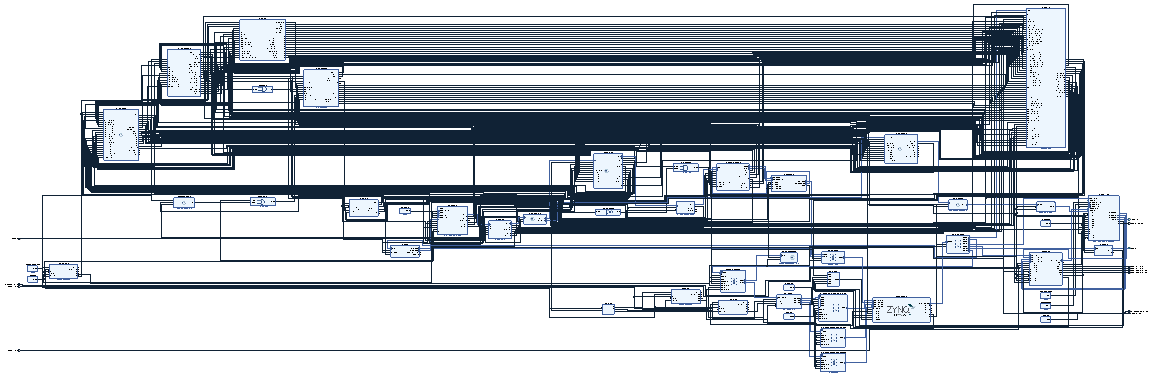
\includegraphics[width=\linewidth,height=0.78\textheight,keepaspectratio]{images/circuits/system_bd.pdf}
    \caption*{附图 A 整机 Block Design 实际连接概览（局部连接见图2-7）}
\end{figure}
\end{landscape}

\end{document}
